\chapter{背景知识}
\label{chap:background}

% Sec 2.1
\section{LBM的起源}
\label{sec:2_LBM_origin}
格子玻尔兹曼方法起源于格子气自动机 (Lattice Gas Automata, LGA) 方法。如方法中的名字所述,LBM继承了方法中格子的概念。LGA依赖于微观方法,在该方法中流体系统使用粒子描述,而非我们一般接触的宏观连续状态量。这些粒子在计算中并不能自由地无规则运动,而有一定的约束。在一个规则网格中,这些粒子只会在网格的相邻节点间迁移,并在格点发生碰撞。在真实世界中,每次碰撞后粒子的速度应该是一个连续的独立变量,并可以先验得到。而因为格子的存在,速度空间只能被离散化,而不再是连续的空间。在一类LGA中,格子可能是六边形的,如图~\ref{img:LGA_lattice} 所示,该类方法被称为FHP方法~\citep{frisch1986lattice},根据三位提出者Frisch、Hasslacher与Pomeau命名。

\begin{figure}[htb]
    \centering
      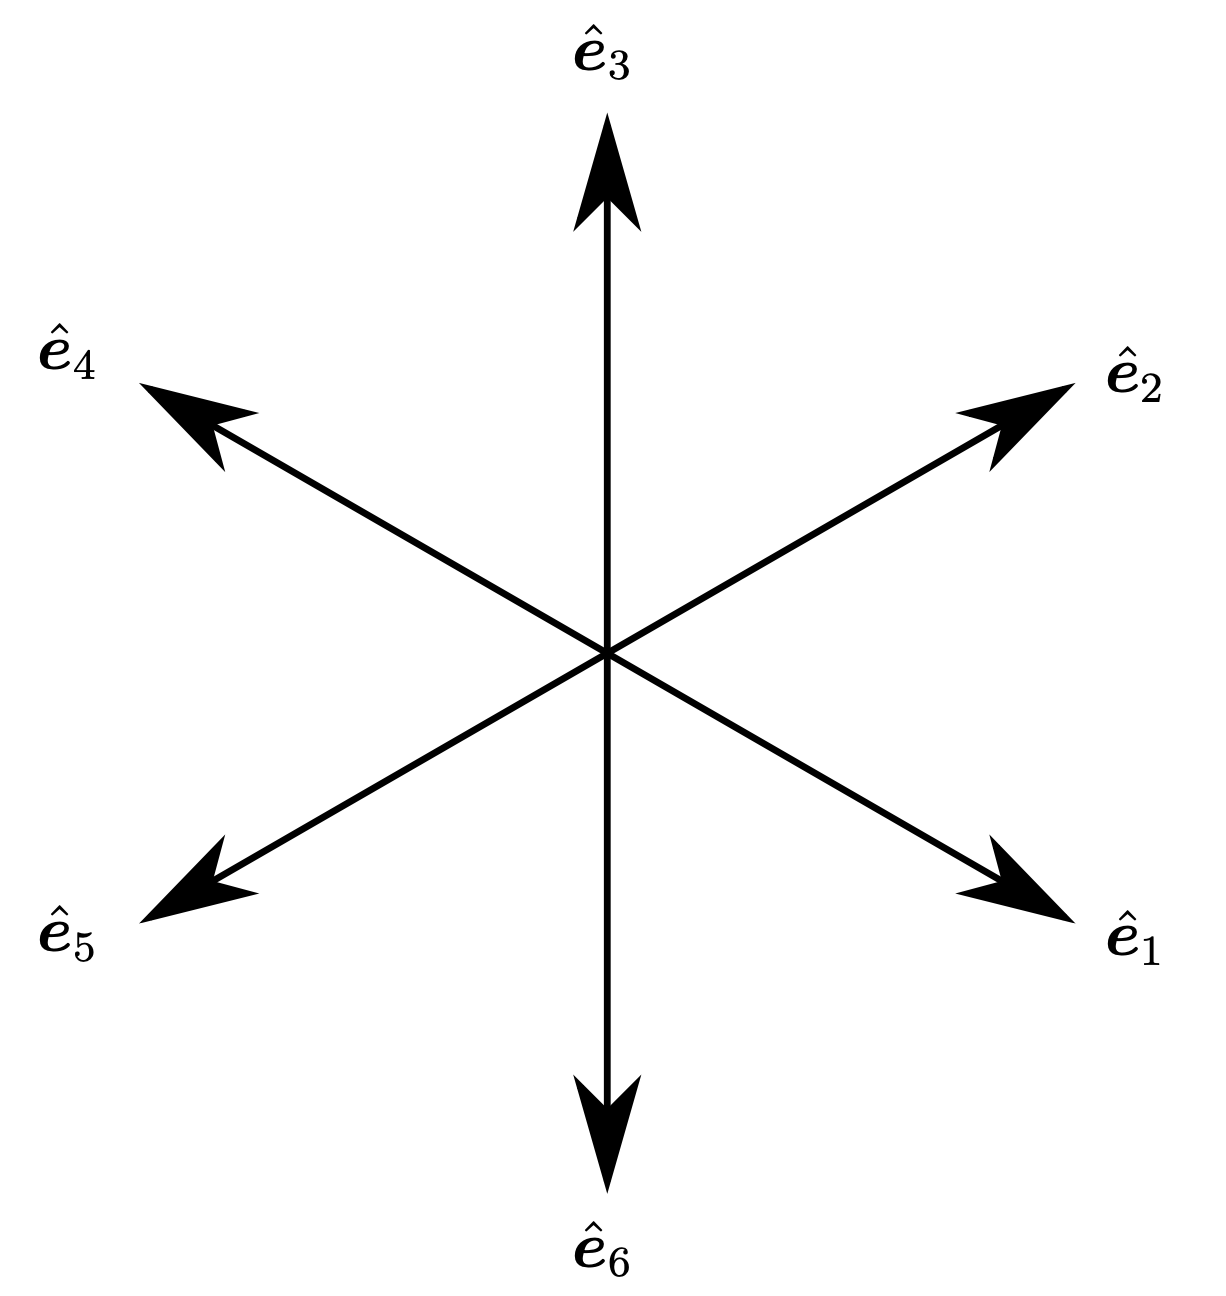
\includegraphics[width=0.5\columnwidth]{figures/LGA_lattice.png}
    \bicaption[二维速度空间中FPH模型的六边形格子]{二维速度空间中FPH模型的六边形格子。其包含有六个离散速度方向。}{Hexagonial lattice of the FHP model with six discrete velocity directions in two-dimensional velocity space.}
    \label{img:LGA_lattice}
\end{figure}

不论LGA或LBM,有一个通用的假设是,在一个时间步长$\Delta t$后,一个粒子会正好走过两个相邻格点间的距离$\Delta x$。对于一个六边形网格,有
\begin{equation}
    \mathbf{c}_i=\frac{\Delta x}{\Delta t}\hat{\mathbf{e}}_i,
\end{equation}
其中$\hat{\mathbf{e}}_i=\mathbf{e}_i/|\mathbf{e}_i|$是归一化后的粒子运动方向,$i$是速度方向的标号,$\mathbf{c}_i$是离散速度。那么接下来可以定义粒子的状态$n_{i}(\mathbf{x},t)$,这个状态值可以是0或1。不考虑碰撞的话,粒子的运动可以用方程描述:
\begin{equation}
    n_{i}(\mathbf{x}+\mathbf{c}_i \Delta t,t+\Delta t)=n_{i}(\mathbf{x},t).
    \label{eq:LGA}
\end{equation}
公式~\ref{eq:LGA} 构成了LGA中标志性的迁移步骤。这一过程也被LBM所继承。这一点为LBM方法带来了很大的优势,首先就是线性的对流项大幅降低了计算难度。其次是这一种直接的空间离散形式并不需要生成一个特殊的计算网格,使前处理的复杂度也能大幅下降。然而这并不代表LBM对网格完全没有要求,这类基于格子的方法只能被应用于六边形或更常见的笛卡尔网格也是一种对网格的约束。

在LGA中,因为粒子只有两种状态,所以经常使用布尔 (Boolean) 变量表示。一般值为真 (true) 时表示在某个空间位置上有一个粒子正在以特定的速度移动,而值为假 (false) 时表示没有这样的粒子。这清楚地显示LGA方法是在粒子层面来表示流体的运动的~\citep{wolf2004lattice}。而很显然,想要完全真实地使用粒子来表示流体是不现实的,因为$1cm^3$的空气中就含有约$2.7\times 10^{19}$个粒子。这导致LGA只能采用比现实情况要低得多的粒子量进行仿真,使结果有很强的噪声,从而LGA需要在空间和时间上进行平均才能取得相对正常的结果。为了解决这一问题,\citet{PhysRevLett.61.2332} 提出使用一个表示粒子密度的分布函数来替代这种单个的粒子。这种抽象的表达也是玻尔兹曼输运方程 (Boltzmann Transport Equation, BTE) 的构成基础。所以被传输的值不再只是一个布尔值,而是一个实数。这个实数表达了在空间位置$\mathbf{x}$、时间$t$,找到一个速度为$\mathbf{c}$的粒子的概率的空间密度。那么在没有碰撞时的迁移步骤的方程变为:
\begin{equation}
    f_{i}(\mathbf{x}+\mathbf{c}_i \Delta t,t+\Delta t)=f_{i}(\mathbf{x},t),
    \label{eq:LBM_streaming}
\end{equation}
其中$f_{i}$是上述的概率分布函数,可以简称为分布函数。一般认为这标志着LBM的诞生。因为在微观过程上使用了统计的概念,所以LBM被称为介观 (mesoscopic) 方法。我们注意在公式~\ref{eq:LGA} 与~\ref{eq:LBM_streaming} 中,我们只考虑了粒子的迁移,而忽略了粒子间的交互。考虑粒子间的交互,这个过程可以表示为
\begin{equation}
    f_{i}(\mathbf{x}+\mathbf{c}_i \Delta t,t+\Delta t)=f_{i}(\mathbf{x},t)+\Omega(f_{i}(\mathbf{x},t)),
    \label{eq:LBM_in_one}
\end{equation}
其中$\Omega$是碰撞运算符 (collision operator)。在实际实现时,我们通常会将公式~\ref{eq:LBM_in_one} 表示为两个分开的过程,即碰撞 (collision) 和迁移 (streaming):
\begin{alignat}{2}
\textbf{碰撞:} & \quad\quad &&f_i^*(\boldsymbol{x}, t) =f_i(\boldsymbol{x}, t)+\Omega\left(f_i(\boldsymbol{x}, t)\right); \\
\textbf{迁移:} & &&f_i\left(\boldsymbol{x}+\mathbf{c}_i \Delta t, t+\Delta t\right) =f_i^*(\boldsymbol{x}, t),\label{eq:LBM_streaming_in_one}
\end{alignat}
其中,$f_i^*$表示碰撞后的分布函数。为了满足质量与动量守恒,LGA中的碰撞中设定了一些固定的规则。对于FHP模型来说,其只允许两个或三个粒子间的碰撞,并且粒子离开格点的方向不能和进入格点的方向一样。这使得两个粒子间的碰撞只有两种可能的结果,而三个粒子间的碰撞只有一种可能的结果,参见图~\ref{img:LGA_collision}。

\begin{figure}[htb]
    \centering
      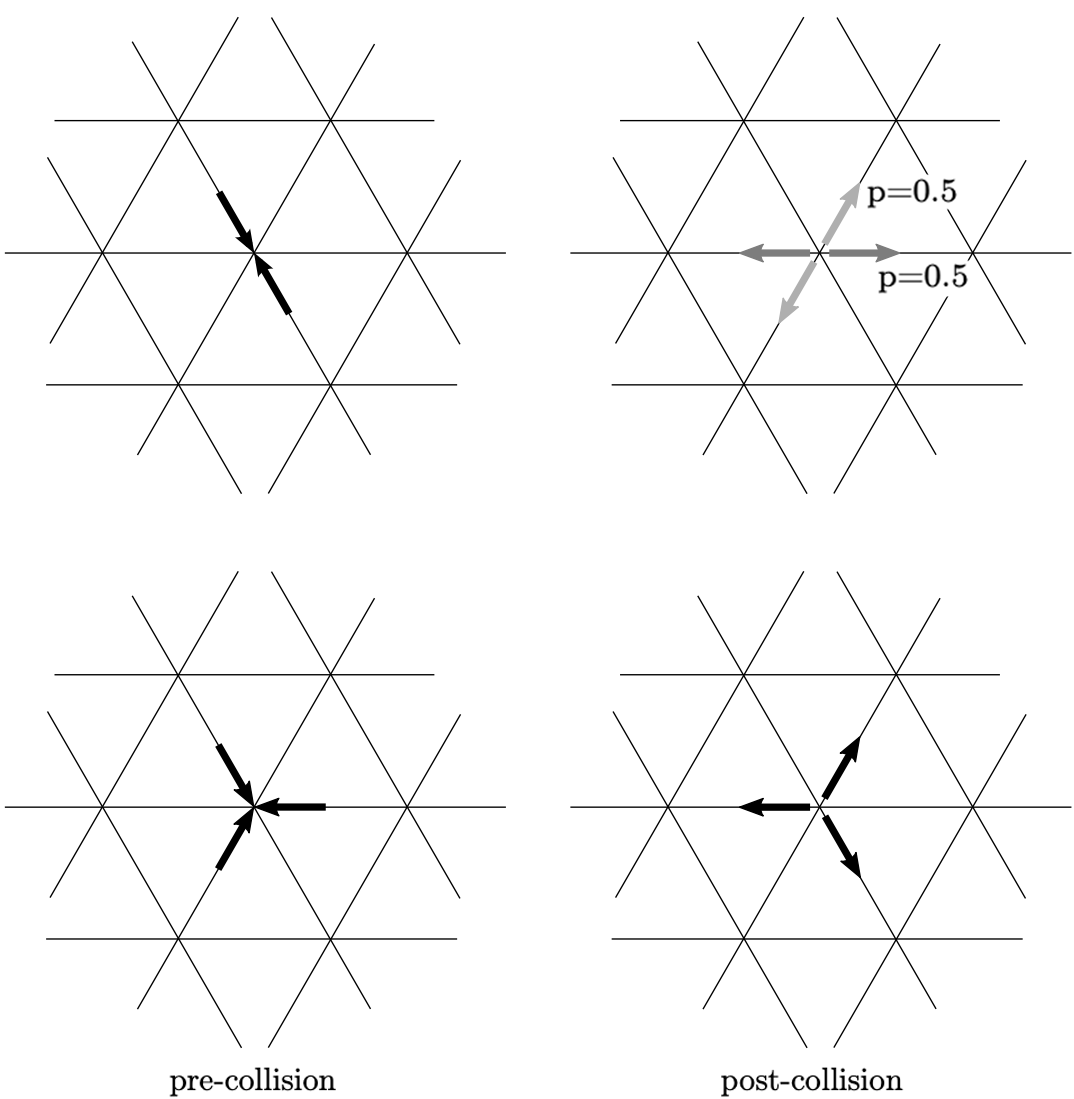
\includegraphics[width=0.84\columnwidth]{figures/LGA_collision.png}
    \bicaption[FHP模型中,两个粒子间的碰撞与三个粒子间的碰撞示意]{FHP模型中,两个粒子间的碰撞与三个粒子间的碰撞示意。$p$表示碰撞后的概率分布。}{Two- and three-particle collision in the FHP model. $p$ denotes the probablility of a particular post-collision state.}
    \label{img:LGA_collision}
\end{figure}

虽然,最初的LBM模型也是基于这些碰撞规则,但是很快人们发现这样的碰撞规则不仅物理上不够精确,对于三维来说,所需的计算量也是不现实的。于是另一种增强的碰撞方案被提出~\citep{higuera1989lattice, higuera1989boltzmann},该方案将非线性的碰撞运算进行了线性化,使碰撞后的值与一个平衡态产生联系:
\begin{equation}
    \Omega(\mathbf{f}(\mathbf{x},t))=\mathbf{A}(\mathbf{f}(\mathbf{x},t)-\mathbf{f}^{eq}(\mathbf{x},t)),
\end{equation}
其中$\mathbf{f}=\{f_i\}$,$\mathbf{f}^{eq}=\{f_{i}^{eq}\}$,$\mathbf{A}$是一个散射矩阵 (scattering matrix),$f_{i}^{eq}$是离散的麦克斯韦-玻尔兹曼平衡态函数 (Maxwell-Boltzmann equilibrium function)。之后~\citet{qian1992lattice} 对碰撞模型进一步简化,基本确定了现在最常见的LBM的碰撞形式,即粒子间的碰撞可以看作是分布函数向平衡态的一个松弛过程:
\begin{equation}
    \mathbf{A}=-\mathbf{I}\tilde{\omega},
\end{equation}
其中$\mathbf{I}$是单位矩阵。
那么这个散射矩阵事实上可以被一个松弛系数 (relaxation rate) $\tilde{\omega}$替代了,这个系数是松弛时间 (relaxation time) $\tilde{\tau}$的倒数:$\tilde{\omega}^{-1}=\tilde{\tau}=\frac{\tau}{\Delta t}$. 从而,公式~\ref{eq:LBM_in_one} 变为
\begin{equation}
    f_{i}(\mathbf{x}+\mathbf{c}_i \Delta t,t+\Delta t)=f_{i}(\mathbf{x},t)-\tilde{\omega}(f_{i}(\mathbf{x},t)-f_{i}^{eq}(\mathbf{x},t)).
    \label{eq:LBM_in_one_BGK}
\end{equation}
公式~\ref{eq:LBM_in_one_BGK} 中,所有的分布函数都以相同的速率向平衡态松弛,虽然这样非常地简洁高效,但是这种方法没有考虑对于分布函数中有物理意义和没有物理意义的部分是否需要分开处理。之后~\citet{d1992generalized} 证明散射矩阵$\mathbf{A}$可以由一组特征基得到,这为多松弛时间模型的出现奠定了基础。

这种对碰撞本身的效果建模,而不是对微观过程建模的想法,最早可见于连续玻尔兹曼方程中的BGK碰撞模型~\citep{Bhatnagar-1954}。这个想法背后的动机是碰撞过程的大部分细节并不会对宏观量产生影响,所以可以将这些过程省略。除了质量与动量守恒之外,BGK模型还满足$\mathrm{H}$-定理 (H-theorem),即分布函数会向平衡态趋近。基于BGK的LBM也是最简洁、最常见的LBM模型。


% Sec 2.2
\section{从介观量到宏观量}
\label{sec:moment}
对于大多数的流体应用,使用一组连续的状态量来描述,如速度、压力等一般已经足够。这些量其实是微观粒子状态的统计平均。在宏观上,流体可以被视为连续体并由N-S方程描述。然而LBM并非是一个宏观方法,而是介于微观与宏观之间的介观层面,如图~\ref{img:fluid_abstraction} 所示。

\begin{figure}[htb]
    \centering
      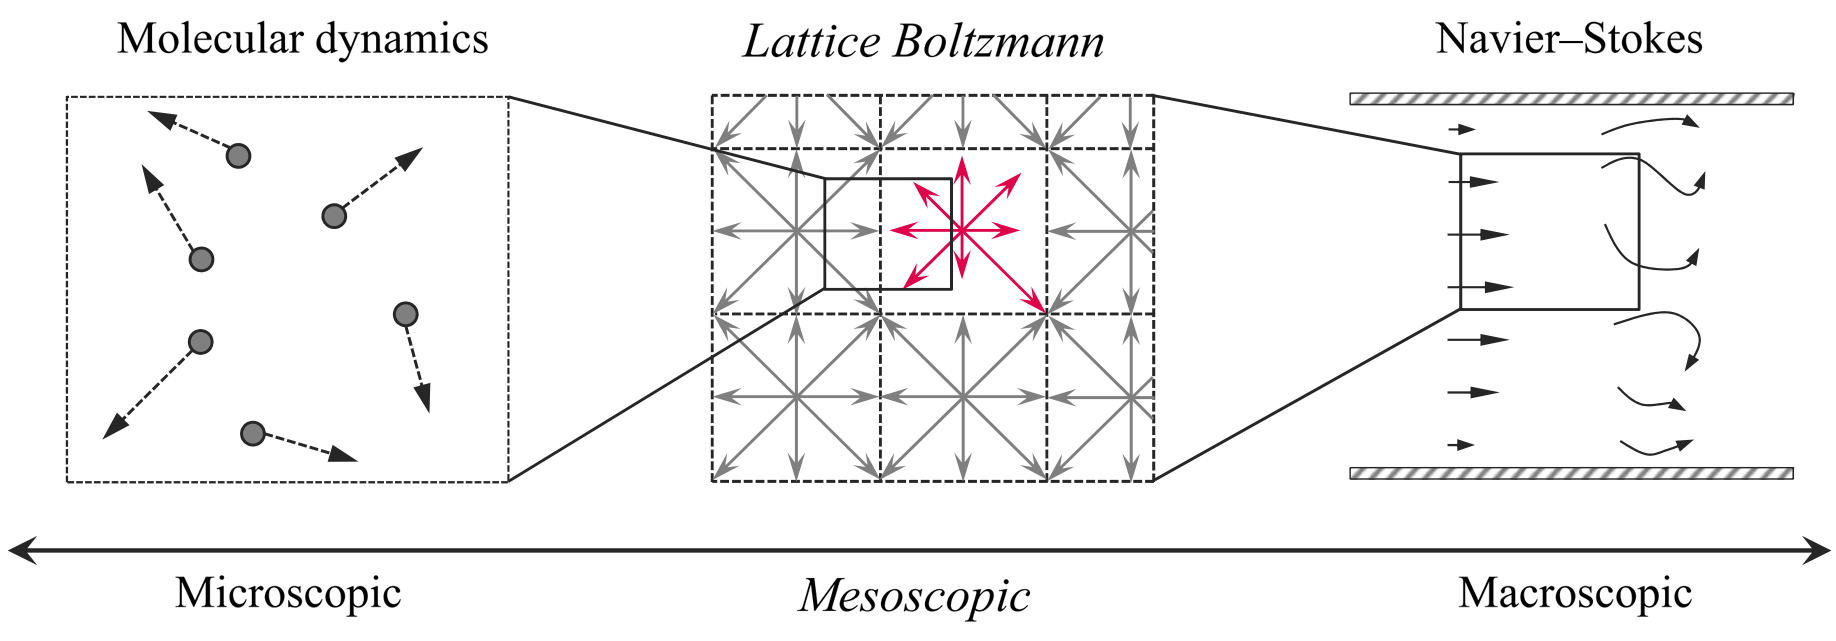
\includegraphics[width=0.99\columnwidth]{figures/fluid_abstraction.png}
    \bicaption[流体力学中的不同抽象层级]{流体力学中的不同抽象层级。格子玻尔兹曼方法被称作介观方法,是介于微观 (如分子动力学) 与宏观 (基于N-S的方法) 之间的层级。图片来自~\citep{PhysRevE.96.013317}。}{Different abstraction levels of the fluid dynamics. The lattice Boltzmann method is the so-called mesoscopic simulation method between the microscopic particle-based (e.g., molecular dynamics) and macroscopic Navier-Stokes-based methods. Image from~\citep{PhysRevE.96.013317}.}
    \label{img:fluid_abstraction}
\end{figure}

可以认为LBM虽然采用了一种非常简化的方案,但它依然计算了部分的微观层面的交互。这也使得LBM的求解过程与N-S方程求解有本质的区别。然而我们最终目的依然是获取宏观的流体状态,以符合我们在宏观世界中对流体的感受。接下来我们将逐步介绍LBM中的概念,并建立其与宏观世界的联系。

可以认为,在一个给定的控制体积 (control volume) 中,分布函数表示了速度在$\mathbf{c}$与$\mathbf{c}+d\mathbf{c}$之间的粒子总数,而宏观现象可以被认为是这一些微观粒子平均后所表达出的现象。所以宏观和介观值可以通过对速度空间$\mathbf{C}$积分来建立联系,通过积分我们可以得到速度的n阶矩
\begin{equation}
    \boldsymbol{M}^{(n)}=\int_{\mathbb{R}^{\mathrm{D}}} \underbrace{\mathbf{c} \mathbf{c} \ldots \mathbf{c}}_{\mathrm{n} \text {次}} f(\boldsymbol{x}, \mathbf{c}, t) \mathrm{d} \mathbf{c},
\end{equation}
这里$D$代表空间的维度。在宏观层面,质量、动量和能量的守恒是由方程自身保证的,然而在介观层面,我们需要通过对碰撞运算符施加约束来保证 (即我们要求碰撞不能破环这些量的守恒),这个约束可以写作
\begin{equation}
    \int\left(\Omega \cdot \psi\right) \mathrm{d} \mathbf{c}=0,
    \label{eq:collision_invariants}
\end{equation}
其中$\psi$是碰撞不变量 (collision invariants)。质量、动量和能量的守恒要求当$\psi=1, \mathbf{c}, \frac{1}{2}|\mathbf{c}|^2$时,公式~\ref{eq:collision_invariants} 是成立的。如果我们将碰撞不变量与分布函数的积进行积分,我们可以自然地得到连续速度空间中的宏观量
\begin{equation}
    \left\{
        \begin{array}
        {l}\rho(\boldsymbol{x}, t)=\int f(\boldsymbol{x}, \mathbf{c}, t) \mathrm{d} \mathbf{c} , \\
        \rho \boldsymbol{u}(\boldsymbol{x}, t)=\int \mathbf{c} f(\boldsymbol{x}, \mathbf{c}, t) \mathrm{d} \mathbf{c} , \\
        \rho E(\boldsymbol{x}, t)=\frac{1}{2} \int|\mathbf{c}|^2 f(\boldsymbol{x}, \mathbf{c}, t) \mathrm{d} \mathbf{c} ,
        \end{array}
    \right.
\end{equation}
其中$E$为比能 (specific energy)。对于单原子气体,碰撞可以假设为弹性的,所以比能包含内能与动能
\begin{equation}
    \rho E=\rho\left(e+\frac{1}{2}|\boldsymbol{u}|^2\right).
\end{equation}
对于本动速度 (peculiar velocity) $\boldsymbol{v}=\mathbf{c}-\boldsymbol{u}$,即粒子在速度为$\boldsymbol{u}$的平均流中的相对速度,我们可以得到类似的公式:
\begin{equation}
    \rho e(\boldsymbol{x}, t)=\frac{1}{2} \int|\boldsymbol{v}|^2 f(\boldsymbol{x}, \mathbf{c}, t) \mathrm{d} \mathbf{c}.
\end{equation}
在连续概念的流体力学中,内能的守恒方程通过一个状态方程$p=p(\rho,e)$将压力和密度联系起来,即
\begin{equation}
    p=\frac{1}{\mathrm{D}} \int|\boldsymbol{v}|^2 f(\boldsymbol{x}, \mathbf{c}, t) \mathrm{d} \mathbf{c}=\frac{2}{\mathrm{D}} \rho e.
    \label{eq:eos}
\end{equation}
对于满足理想气体定律 (perfect gas law) 的等温流体,可以得到
\begin{equation}
    e=\frac{\mathrm{D}}{2} \frac{p}{\rho}=\frac{\mathrm{D}}{2} R T_0=\frac{\mathrm{D}}{2} \frac{k_B T_0}{m}=\frac{\mathrm{D}}{2} c_s^2,
\end{equation}
其中$T_0$和$c_s$分别表示常值的温度与声速,$k_B$是玻尔兹曼常数 (Boltzmann constant),$R$是气体常数 (gas constant),$m$是气体粒子的平均质量。所以公式~\ref{eq:eos}可以被重写为
\begin{equation}
    p=\rho c_s^2,
\end{equation}
即绝热系数$\gamma=1$时的等熵状态方程~\citep{kundu2015fluid}。这样我们也通过密度建立了介观量与压力间的联系。

% Sec 2.3
\section{速度空间的离散化}
如前文所述,由于在求解时保留了格子的概念,所以我们必须类似地对速度空间进行离散。分布函数事实上可以表达为Hermite (埃尔米特) 多项式构成的无穷级数,变量为经过声速正则化后的速度空间$\tilde{\mathbf{c}}=\mathbf{c}/c_s$:
\begin{equation}
    f(\boldsymbol{x}, \mathbf{c}, t)=\frac{1}{c_s^{\mathrm{D}}} \omega(\tilde{\mathbf{c}}) \sum_{n=0}^{\infty} \frac{1}{n !} \boldsymbol{a}^{(n)}(\boldsymbol{x}, t) \mathscr{H}^{(n)}(\tilde{\mathbf{c}}),
    \label{eq:hermite_f}
\end{equation}
其中$\mathscr{H}^{(n)}$是$n$次Hermite多项式。Hermite多项式的一个特点是展开系数$\boldsymbol{a}^{(n)}$是$f$本身的速度矩~\citep{shan2006kinetic},权重函数$\omega$为
\begin{equation}
    \omega(\tilde{\mathbf{c}})=\frac{1}{(2 \pi)^{\mathrm{D} / 2}} \exp \left(-\tilde{\mathbf{c}}^2 / 2\right).
\end{equation}
当流体不受压力时,流体可以被一个平衡态函数描述。这只会出现在密度和速度在整个流体域中都是常值的情况下。此时的平衡态可由麦克斯韦分布函数描述
\begin{equation}
    f^{eq}=\frac{\rho}{\left(2 \pi c_s^2\right)^{\mathrm{D} / 2}} \exp \left(\frac{-(\mathbf{c}-\boldsymbol{u})^2}{2 c_s^2}\right),
    \label{eq:maxwell_eq}
\end{equation}
其中$\rho$和$\boldsymbol{u}$分别为宏观的密度和速度。我们可以将这个平衡态函数投影到基为Hermite多项式的空间,此时速度矩变为$\boldsymbol{a}^{eq,(n)}$:
\begin{equation}
    f^{eq}(\boldsymbol{x}, \mathbf{c}, t)=\frac{1}{c_s^{\mathrm{D}}} \omega(\tilde{\mathbf{c}}) \sum_{n=0}^{\infty} \frac{1}{n !} \boldsymbol{a}^{eq,(n)}(\boldsymbol{x}, t) \mathscr{H}^{(n)}(\tilde{\mathbf{c}}).
    \label{eq:maxwell_eq_hermite}
\end{equation}
对比公式~\ref{eq:hermite_f},我们可以注意到两式几乎有着相同的形式。事实上,$f^{eq}$还可表达为
\begin{equation}
    f^{eq}=\frac{\rho}{c_s^D}\omega(\tilde{\boldsymbol{v}}),
\end{equation}
其中$\tilde{\boldsymbol{v}}=(\mathbf{c}-\mathbf{u})/c_s$可视为本动马赫数。所以麦克斯韦分布函数的Hermite展开系数为
\begin{equation}
    \boldsymbol{a}^{eq,(n)}=\rho \int w(\tilde{\boldsymbol{v}}) \mathscr{H}^{(n)}\left(\tilde{\boldsymbol{v}}+\frac{\boldsymbol{u}}{c_s}\right) \mathrm{d} \tilde{\boldsymbol{v}}.
    \label{eq:hermite_coefficients}
\end{equation}
对公式~\ref{eq:hermite_f} 这样的无穷级数进行截断,即对应着对速度空间的离散化,并且保证了连续空间和离散空间下的矩在截断的阶数$N$前是不变的。而离散的一个重要约束来自于高斯积分
\begin{equation}
    \int \omega(\boldsymbol{x}) f(\boldsymbol{x}) \mathrm{d} \boldsymbol{x} \approx \sum \omega_i f(\boldsymbol{x}_i), \quad i=0,1, \ldots, q-1
\end{equation}
其中,$f(\boldsymbol{x})$可表示任意函数而$\omega_i$是常值的权重。
%我们用$\tilde{{c}}_i$表达在$N$阶截断后的Hermite级数的横坐标 (abscissae),则高阶的截断一定会需要更多数量的离散速度,使格子的拓扑更难构造。
我们可以将高斯积分的公式抽象地记为$E^q_{D,n}$,
其中$D$表示空间的维度,$n$为积分代数精度的阶数,$q$表示积分所需要的离散点的数量。则我们可以推导出这三个值间的关系。对于一维空间,首先一个通用的约束为$n>2N$,即我们若要保持在$N=2$阶时,离散的矩与原始矩相同,我们至少需要积分代数精度为$n=5$阶~\citep{shan2006kinetic}。在一维空间中,高斯积分有$n=2q-1$的关系,所以可得$q=3$。对于高维空间并没有一般的高斯积分理论,但是维持积分代数精度为$n=5$阶时且格子为笛卡尔网格时,二维空间至少需要9个离散速度,三维空间时至少需要15个。如果依然采用~\citep{qian1992lattice}中的D$d$Q$q$的命名法的话 ($d$表示空间维度,$q$表示离散速度个数),能维持二阶精度的格子分别为D1Q3、D2Q9、D3Q15。由公式~\ref{eq:hermite_coefficients} 可得,在截断至二阶时,Hermite展开的系数为
\begin{equation}
    \left\{\begin{array}{l}\boldsymbol{a}^{eq, 0}=\rho \\ \boldsymbol{a}^{eq, 1}=\rho \frac{\boldsymbol{u}}{c_s} \\ \boldsymbol{a}^{eq, 2}=\rho \frac{u_i u_j}{c_s^2}\end{array}\right.
\end{equation}
将其代入到公式~\ref{eq:maxwell_eq_hermite}中,可以得到
\begin{equation}
    f_i^{eq}(\boldsymbol{x}, t)=w_i \rho\left(1+\frac{\mathbf{c}_i \cdot \boldsymbol{u}}{c_s^2}+\frac{\left(\mathbf{c}_i \cdot \boldsymbol{u}\right)^2}{2 c_s^4}-\frac{u^2}{2 c_s^2}\right),
    \label{eq:f_eq_o2}
\end{equation}
其中$f_i^{eq}(\boldsymbol{x}, t)=f^{eq}(\boldsymbol{x}, {c}_i, t)$, $\omega_i=\omega(\frac{\mathbf{c}}{c_s})/c_s^D$。上述的推导尝试在尽量保持简洁的前提下,用比较系统且严格的形式推导出分布函数及速度空间的离散,所以无法过于详尽地展示出所有步骤。对于更彻底的推导,读者们可以参考~\citep{shan2006kinetic, malaspinas2010lattice}。


% Sec 2.4
\section{从LBM到N-S方程}
\label{sec:lbm_to_ns}
在介绍过速度矩作为介观和宏观世界之间的联系之后,我们现在将使用多尺度分析 (multiple-scale analysis) 来从LBE推导出N-S方程。许多流体的动态特征其实表现于其与平衡态的偏移。如果在介观上,分布函数都处于平衡态,那么可以想像,在宏观上流体也是平静的。所以多尺度分析的思想是将$f$在$f^{eq}$处展开。展开后的$f^{eq}$可以被记为$f^{(0)}$,其余部分为非平衡态项:
\begin{equation}
    f=\underbrace{f^{(0)}}_{f^{e q}}+\underbrace{\epsilon f^{(1)}+\epsilon^2 f^{(2)}}_{f^{n e q}} \cdots .
\end{equation}
多尺度分析的扩展依赖于一个很小的参数$\epsilon$,这个值是松弛时间$\tau=\nu/c_s^2$与格子时间步长$\Delta t$的比值。对流的时间尺度 (advection timescale) 是直接与$\Delta t_1=\tau/\epsilon$联系的,而粘性扩散的时间尺度 (viscous diffusion timescale) 是联系于
\begin{equation}
    \Delta t_2=\frac{\Delta x^2}{\nu} \sim \frac{c_s^2 \Delta t^2}{\nu}=\frac{\tau}{\epsilon^2}
    \label{eq:ms_f}
\end{equation}
的。有推导证明我们将$f$展开到一阶 ($\epsilon f^{(1)}$) 时,可以推导出欧拉方程~\citep{huang2008statistical}。为了推导N-S方程,我们需要展开到二阶 (即$\epsilon^2 f^{(2)}$),此时时间上的导数运算符为
\begin{equation}
    \frac{\partial}{\partial t}=\epsilon \frac{\partial}{\partial t_1}+\epsilon^2 \frac{\partial}{\partial t_2},
    \label{eq:ms_t}
\end{equation}
空间上的导数运算符为
\begin{equation}
    \frac{\partial}{\partial \boldsymbol{x}}=\epsilon \frac{\partial}{\partial \boldsymbol{x}_1}.
    \label{eq:ms_x}
\end{equation}
在将$f$分解为平衡态与非平衡态后,公式~\ref{eq:collision_invariants} 所表达的约束可被表达为
\begin{equation}
    \left\{\begin{array}{l}\sum_{i} f_{i}^{(n)}=0 \\ \sum_{i} \mathbf{c}_{i} f_{i}^{(n)}=\mathbf{0}\end{array}\right., \quad  n=1,2, \ldots.
\end{equation}
那么为了将LBE恢复到N-S方程,首先我们要将公式~\ref{eq:LBM_in_one_BGK} 的左手侧进行二阶的泰勒 (Taylor) 展开
\begin{align}
    \begin{split}
        & f_{i}\left(\boldsymbol{x}+\mathbf{c}_{i} \Delta t, t+\Delta t\right) \approx \\
        & \quad f_{i}(\boldsymbol{x}, t)+\left({c}_{i \alpha} \Delta t \frac{\partial}{\partial x_{\alpha}}+\Delta t \frac{\partial}{\partial t}\right) f_{i}(\boldsymbol{x}, t)+ \\
        & \quad \frac{1}{2}\left({c}_{i \alpha} {c}_{i \beta} \Delta t^{2} \frac{\partial^{2}}{\partial x_{\alpha} \partial x_{\beta}}+2 {c}_{i \alpha} \Delta t^{2} \frac{\partial}{\partial x_{\alpha}} \frac{\partial}{\partial t}+\Delta t^{2} \frac{\partial^{2}}{\partial t^{2}}\right) f_{i}(\boldsymbol{x}, t)+\mathcal{O}\left(\Delta t^{3}\right) .
    \end{split}
    \label{eq:ms_taylor}
\end{align}
我们将上式代入公式~\ref{eq:LBM_in_one_BGK},并用$\tau$替代$\tilde{\omega}$后,可以得到
\begin{equation}
\Delta t\left({c}_{i \alpha} \frac{\partial}{\partial x_{\alpha}}+\frac{\partial}{\partial t}\right) f_{i}+\frac{\Delta t^{2}}{2}\left({c}_{i \alpha} {c}_{i \beta} \frac{\partial^{2}}{\partial x_{\alpha} \partial x_{\beta}}+2 {c}_{i \alpha} \frac{\partial}{\partial x_{\alpha}} \frac{\partial}{\partial t}+\frac{\partial^{2}}{\partial t^{2}}\right) f_{i}=-\frac{\Delta t}{\tau}\left(f_{i}-f_{i}^{e q}\right) .
\end{equation}
接下来,我们将多尺度分析的公式~\ref{eq:ms_f} 至~\ref{eq:ms_x} 代入上式
\begin{align}
    \begin{split}
& {\left[{c}_{i \alpha}\left(\epsilon \frac{\partial}{\partial x_{1 \alpha}}\right)+\left(\epsilon \frac{\partial}{\partial t_{1}}+\epsilon^{2} \frac{\partial}{\partial t_{2}}\right)\right]\left(f_{i}^{(0)}+\epsilon f_{i}^{(1)}+\epsilon^{2} f_{i}^{(2)}\right)+} \\
& \frac{\Delta t}{2}\left[{c}_{i \alpha} {c}_{i \beta}\left(\epsilon^{2} \frac{\partial^{2}}{\partial x_{1 \alpha} \partial x_{1 \beta}}\right)+\left(2 {c}_{i \alpha} \epsilon^{2} \frac{\partial}{\partial x_{1 \alpha}} \frac{\partial}{\partial t_{1}}\right)+\left(\epsilon^{2} \frac{\partial^{2}}{\partial t_{1}^{2}}\right)\right]\left(f_{i}^{(0)}+\epsilon f_{i}^{(1)}+\epsilon^{2} f_{i}^{(2)}\right)= \\
& \quad-\frac{1}{\tau}\left(f_{i}^{(0)}+\epsilon f_{i}^{(1)}+\epsilon^{2} f_{i}^{(2)}-f_{i}^{e q}\right) .
    \end{split}
    \label{eq:ms_total}
\end{align}
然后,我们把公式~\ref{eq:ms_total} 按照$\epsilon$的阶数分离:

\noindent
$\mathcal{O}\left(\epsilon^{0}\right):$
\begin{equation}
f_{i}^{(0)}=f_{i}^{e q}
\end{equation}
$\mathcal{O}\left(\epsilon^{1}\right):$
\begin{equation}
\epsilon\left({c}_{i \alpha} \frac{\partial}{\partial x_{1 \alpha}}+\frac{\partial}{\partial t_{1}}\right) f_{i}^{(0)}=-\frac{1}{\tau} \epsilon f_{i}^{(1)}
\label{eq:ms_o1}
\end{equation}
$\mathcal{O}\left(\epsilon^{2}\right):$
\begin{equation}
\epsilon^{2} \frac{\partial}{\partial t_{2}} f_{i}^{(0)}+\left({c}_{i \alpha} \epsilon \frac{\partial}{\partial x_{1 \alpha}}+\epsilon \frac{\partial}{\partial t_{1}}\right) \epsilon f_{i}^{(1)}+\frac{\Delta t}{2}\left({c}_{i \alpha} \epsilon \frac{\partial}{\partial x_{1 \alpha}}+\epsilon \frac{\partial}{\partial t_{1}}\right)^{2} f_{i}^{(0)}=-\frac{1}{\tau} \epsilon^{2} f_{i}^{(2)} .
\label{eq:ms_o2}
\end{equation}
将公式~\ref{eq:ms_o1} 代入公式~\ref{eq:ms_o2},可以得到
\begin{equation}
\epsilon^{2} \frac{\partial}{\partial t_{2}} f_{i}^{(0)}+\left({c}_{i \alpha} \epsilon \frac{\partial}{\partial x_{1 \alpha}}+\epsilon \frac{\partial}{\partial t_{1}}\right)\left(1-\frac{\Delta t}{2 \tau}\right) \epsilon f_{i}^{(1)}=-\frac{1}{\tau} \epsilon^{2} f_{i}^{(2)} .
\label{eq:ms_o1_into_o2}
\end{equation}
接下来我们想要获得关于宏观量的守恒公式,与求矩类似,我们对公式~\ref{eq:ms_o1} 与公式~\ref{eq:ms_o1_into_o2} 对碰撞不变量积分得到0阶与1阶的矩公式
\begin{equation}
\epsilon \frac{\partial \rho}{\partial t_{1}}+\epsilon \frac{\partial \rho u_{\alpha}}{\partial x_{1 \alpha}}=0 ,
\label{eq:ms_moment_o1_a}
\end{equation}
\begin{equation}
\epsilon \frac{\partial \rho u_{\alpha}}{\partial t_{1}}+\epsilon \frac{\partial P_{\alpha \beta}^{(0)}}{\partial x_{1 \beta}}=0 .
\label{eq:ms_moment_o1_b}
\end{equation}
同样地,我们对公式~\ref{eq:ms_o2}积分得到矩公式
\begin{equation}
\epsilon^{2} \frac{\partial \rho}{\partial t_{2}} = 0 ,
\label{eq:ms_moment_o2_a}
\end{equation}
\begin{equation}
\epsilon^{2} \frac{\partial \rho u_{\alpha}}{\partial t_{2}} +\left(1-\frac{\Delta t}{2 \tau}\right) \epsilon^{2} \frac{P_{\alpha \beta}^{(1)}}{\partial x_{1 \beta}}=0 .
\label{eq:ms_moment_o2_b}
\end{equation}
然后我们将公式~\ref{eq:ms_moment_o1_a} 与~\ref{eq:ms_moment_o1_b} 相加,并将展开的求导运算符重新代回原式 (参见公式~\ref{eq:ms_t} 与~\ref{eq:ms_x}) 可以得到
\begin{equation}
\frac{\partial \rho}{\partial t}+\frac{\partial \rho u_{\alpha}}{\partial x_{\alpha}}=0,
\end{equation}
即连续性方程。同样将公式~\ref{eq:ms_moment_o2_a} 与~\ref{eq:ms_moment_o2_b} 相加后得到
\begin{equation}
\frac{\partial \rho u_{\alpha}}{\partial t}+\frac{\partial}{\partial x_{\beta}}\left[P_{\alpha \beta}^{e q}+\left(1-\frac{\Delta t}{2 \tau}\right) P_{\alpha \beta}^{n e q}\right]=0,
\label{eq:ms_continuity_puzzle}
\end{equation}
其中$P_{\alpha \beta}^{e q}=P_{\alpha \beta}^{(0)}$,$P_{\alpha \beta}^{n e q}=P_{\alpha \beta}^{(1)}$。
由公式~\ref{eq:f_eq_o2} 我们可以由下面的方式得到二阶矩
\begin{equation}
P_{\alpha \beta}^{(0)}=P_{\alpha \beta}^{e q}=\sum_{\alpha} f_{i}^{e q} {c}_{i, \alpha} {c}_{i, \beta}=\rho c_{s}^{2}\delta_{\alpha \beta}+\rho u_{\alpha} u_{\beta}
\end{equation}
与三阶矩
\begin{equation}
Q_{\alpha \beta \gamma}^{(0)}=Q_{\alpha \beta \gamma}^{e q}=\sum_{\alpha} f_{i}^{e q} {c}_{i, \alpha} {c}_{i, \beta} {c}_{i, \gamma}=\rho c_{s}^{2}\left(u_{\alpha} \delta_{\beta \gamma}+u_{\beta} \delta_{\alpha \gamma}+u_{\gamma} \delta_{\alpha \beta}\right).
\end{equation}
那么在公式~\ref{eq:ms_continuity_puzzle} 中,只剩下$P_{\alpha \beta}^{n e q}$是未知的。为了计算$P_{\alpha \beta}^{n e q}$,我们写出公式~\ref{eq:ms_o1} 的2阶矩公式
\begin{equation}
\epsilon \frac{\partial P_{\alpha \beta}^{(0)}}{\partial t_{1}}+\epsilon \frac{\partial Q_{\alpha \beta \gamma}^{(0)}}{\partial x_{1 \gamma}}=-\frac{1}{\tau} \epsilon P_{\alpha \beta}^{(1)}.
\label{eq:ms_moment_o2}
\end{equation}
接下来,我们引入如下的积分公式 (乘积法则):
\begin{align}
\epsilon \frac{\partial \rho u_{\alpha} u_{\beta}}{\partial t_{1}} & =u_{\alpha} \epsilon \frac{\rho u_{\beta}}{\partial t_{1}}+u_{\beta} \epsilon \frac{\rho u_{\alpha}}{\partial t_{1}}-u_{\alpha} u_{\beta} \epsilon \frac{\partial \rho}{\partial t_{1}}, \\
\epsilon \frac{\partial \rho u_{\alpha} u_{\beta} u_{\gamma}}{\partial x_{1 \gamma}} & =u_{\alpha} \epsilon \frac{\rho u_{\beta} u_{\gamma}}{\partial x_{1 \gamma}}+u_{\beta} \epsilon \frac{\rho u_{\alpha} u_{\gamma}}{\partial x_{1 \gamma}}-u_{\alpha} u_{\beta} \epsilon \frac{\partial \rho u_{\gamma}}{\partial x_{1 \gamma}} .
\end{align}
使用上述的公式,公式~\ref{eq:ms_moment_o2} 左手边的$\epsilon \frac{\partial P_{\alpha \beta}^{(0)}}{\partial t_{1}}$可以被表达为
\begin{align}
    \begin{split}
\epsilon \frac{\partial P_{\alpha \beta}^{(0)}}{\partial t_{1}}= & \epsilon \frac{\partial \rho u_{\alpha} u_{\beta}}{\partial t_{1}}+c_{s}^{2} \delta_{\alpha \beta} \epsilon \frac{\partial \rho}{\partial t_{1}} \\
= & u_{\alpha} \epsilon \frac{\partial \rho u_{\beta}}{\partial t_{1}}+u_{\beta} \epsilon \frac{\partial \rho u_{\alpha}}{\partial t_{1}}-u_{\alpha} u_{\beta} \epsilon \frac{\partial \rho}{\partial t_{1}}+c_{s}^{2} \delta_{\alpha \beta} \epsilon \frac{\partial \rho}{\partial t_{1}} \\
= & -u_{\alpha} \epsilon \frac{\partial P_{\beta \gamma}^{(0)}}{\partial x_{1 \gamma}}-u_{\beta} \epsilon \frac{\partial P_{\alpha \gamma}^{(0)}}{\partial x_{1 \gamma}}+u_{\alpha} u_{\beta} \epsilon \frac{\partial \rho u_{\gamma}}{\partial x_{1 \gamma}}-c_{s}^{2} \delta_{\alpha \beta} \epsilon \frac{\partial \rho u_{\gamma}}{\partial x_{1 \gamma}} \quad \text {(由公式~\ref{eq:ms_moment_o1_a}、\ref{eq:ms_moment_o1_b})} \\
= & -u_{\alpha} \epsilon \frac{\partial}{\partial x_{1 \gamma}}\left(\rho u_{\beta} u_{\gamma}+\rho c_{s}^{2} \delta_{\beta \gamma}\right)-u_{\beta} \epsilon \frac{\partial}{\partial x_{1 \gamma}}\left(\rho u_{\alpha} u_{\gamma}+\rho c_{s}^{2} \delta{\alpha \gamma}\right) \\
& +u_{\alpha} u_{\beta} \epsilon \frac{\partial \rho u_{\gamma}}{\partial x_{1 \gamma}}-c_{s}^{2} \delta_{\alpha \beta} \frac{\partial \rho u_{\gamma}}{\partial x_{1 \gamma}} \\
= & -\epsilon \frac{\partial \rho u_{\alpha} u_{\beta} u_{\gamma}}{\partial x_{1 \gamma}}-c_{s}^{2}\left(u_{\alpha} \epsilon \frac{\partial \rho}{\partial x_{1 \beta}}+u_{\beta} \epsilon \frac{\partial \rho}{\partial x_{1 \alpha}}\right)-c_{s}^{2} \delta_{\alpha \beta} \epsilon \frac{\partial \rho u_{\gamma}}{\partial x_{1 \gamma}} .
    \end{split}
\end{align}
同时,$\epsilon \frac{\partial Q_{\alpha \beta \gamma}^{(0)}}{\partial x_{1 \gamma}}$可表达为
\begin{align}
    \begin{split}
\epsilon \frac{\partial Q_{\alpha \beta \gamma}^{(0)}}{\partial x_{1 \gamma}} & =\epsilon \frac{\partial}{\partial x_{1 \gamma}} \rho c_{s}^{2}\left(u_{\alpha} \delta_{\beta \gamma}+u_{\beta} \delta{\alpha \gamma}+u_{\gamma} \delta_{\alpha \beta}\right) \\
& =c_{s}^{2}\left(\epsilon \frac{\partial \rho u_{\alpha}}{\partial x_{1 \beta}}+\epsilon \frac{\partial \rho u_{\beta}}{\partial x_{1 \alpha}}\right)+c_{s}^{2} \delta_{\alpha \beta} \epsilon \frac{\partial \rho u_{\gamma}}{\partial x_{1 \gamma}}.
    \end{split}
\end{align}
将上述两公式相加可得到$P_{\alpha \beta}^{(1)}$的表达式
\begin{equation}
\epsilon P_{\alpha \beta}^{(1)}=-\rho c_{s}^{2} \tau\left(\epsilon \frac{\partial u_{\alpha}}{\partial x_{1 \beta}}+\epsilon \frac{\partial u_{\beta}}{\partial x_{1 \alpha}}\right)+\tau \epsilon \frac{\partial \rho u_{\alpha} u_{\beta} u_{\gamma}}{\partial x_{1 \gamma}}.
\end{equation}
将 $P^{n e q}=\epsilon P^{(1)}$,$\partial / \partial \boldsymbol{x}=\epsilon \partial / \partial \boldsymbol{x}_{1}$代入,我们可以获得
\begin{equation}
P_{\alpha \beta}^{n e q}=\underbrace{-\rho c_{s}^{2} \tau\left(\frac{\partial u_{\alpha}}{\partial x_{\beta}}+\frac{\partial u_{\beta}}{\partial x_{\alpha}}\right)}_{\text{粘性应力张量}\boldsymbol{\sigma}^{\prime}}+\underbrace{\tau \frac{\partial \rho u_{\alpha} u_{\beta} u_{\gamma}}{\partial x_{k}}}_{\text {误差项}} .
\label{eq:p_neq}
\end{equation}
从上式中我们可以发现,第一项对应于N-S方程中的粘性应力张量 (viscous stress tensor) $\boldsymbol{\sigma}^{\prime}$,而第二项是误差项。因为平衡态函数$f_i^{eq}$只展开到了二阶,所以$\mathcal{O}\left(u^{3}\right)$项是不正确的。当我们仔细观察公式~\ref{eq:p_neq} 时,我们发现当${u_x}^{2} \ll c_{s}^{2}$时,$\mathcal{O}\left(u^{3}\right)$项的模值相比前一项就可以被忽略了。所以在低马赫数时,我们可以直接忽略上式中的误差项。这也是为什么许多工作描述LBM只在弱可压 (weakly compressible) 情况下有效,而不能直接应用于强可压 (strongly compressible) 现象,因为强可压现象发生在跨声速或超声速时,此时误差是不能直接忽略的。
那么我们将忽略误差项的公式~\ref{eq:p_neq} 代入公式~\ref{eq:ms_continuity_puzzle} 后,可以得到动量守恒方程
\begin{equation}
    \frac{\partial \rho u_{\alpha}}{\partial t}+\frac{\partial \rho u_{\alpha} u_{\beta}}{\partial x_{\beta}}=-\frac{\partial p}{\partial x_{\alpha}}+\mu \frac{\partial}{\partial x_{\beta}}\left(\frac{\partial u_{\alpha}}{\partial x_{\beta}}+\frac{\partial u_{\beta}}{\partial x_{\alpha}}\right),
\end{equation}
其中$\mu=\left(1-\frac{\Delta t}{2 \tau}\right) \rho c_{s}^{2} \tau$是动力黏度 (dynamic viscosity),运动黏度 (kinematic viscosity) $\nu=\mu / \rho$与松弛时间$\tau$之间的关系为
\begin{equation}
    \nu=c_{s}^{2}\left(\tau-\frac{\Delta t}{2}\right) \quad \text {或} \quad \tau=\frac{\nu}{c_{s}^{2}}+\frac{\Delta t}{2} .
\end{equation}
因为我们在公式~\ref{eq:ms_taylor} 中对LBE进行了二阶的泰勒展开,所以我们认为在时间和空间上LBM可以以二阶的精度推导出N-S方程。


% Sec 2.5
\section{碰撞模型}
\label{sec:bg_collision}
我们回顾碰撞模型的作用是模拟粒子间的交互,这种交互会使得分布函数向平衡态松弛。在第~\ref{sec:2_LBM_origin} 节的末尾,我们介绍了LBM中的BGK碰撞模型,因为BGK模型需要对所有的分布函数使用相同的速率进行松弛,所以又可以被称为即单松弛时间 (single-relaxation-time) 模型。然而这是BGK模型一个很大的局限性,因为分布函数中非守恒的部分并不需要以同样的速率松弛。而且取决于初始条件与边界条件,这样的松弛方法可能会产生短波震荡,使得低黏度区域的数值稳定性差。所以多松弛时间模型被提出,以克服这些问题。其主要的目的是将分布函数投影至各个维度更为独立的空间中,再完成松弛过程。这个空间由一系列的特征向量构成。在本节中我们将主要介绍不同构造形式的多松弛时间模型。

我们在第~\ref{sec:1_related_works_LBM} 节中介绍了不同的碰撞模型及其发展过程。由于数量众多,我们无法详细介绍所有的碰撞模型,于是在本节中我们主要介绍与我们工作最相关的几种碰撞模型,分别为原始矩、中心矩、自适应中心矩与累积量碰撞模型。

\subsection{原始矩与中心矩碰撞模型}
\label{sec:background_mrt}
我们已经提过MRT碰撞模型的动机是将分布函数投影至由一组特征向量定义的空间中进行松弛操作。依据连续的流体力学理论,最方便的构造这样空间的方法是从三个正交子空间入手,分别是守恒 (conserved) 量空间、传输 (transport) 量空间与虚拟 (ghost) 量空间。其中守恒量对应质量与动量,传输量对应动量通量,虚拟量则没有固定的物理意义。
我们发现这与我们第~\ref{sec:moment} 节中介绍的速度矩的概念十分相近,所以我们可以从速度矩出发来构造这样的空间。这样从绝对的速度矩构造的碰撞模型也被称为也被称作原始矩碰撞模型。从分布函数到矩的转换可以写作$\mathbf{m}=\mathbf{M}\mathbf{f}$,其中$\mathbf{M}=[\mathbf{M}_0, \mathbf{M}_1, \dots, \mathbf{M}_{q-1}]$是分布函数到矩的变换矩阵,$q$为离散速度的数量。从这里开始,没有特殊说明时,本文都考虑D3Q27,即三维下$q=27$时的情况,因为此时的格子在三维中有着最好的对称性。对于原始矩,我们使用~\citep{PhysRevE.95.013310} 中的构造形式
\begin{align*}
    & \boldsymbol{M}_0=\left\{\left\|\boldsymbol{c}_i\right\|^0\right\}, \\
    & \boldsymbol{M}_1=\left\{\boldsymbol{c}_{i, x}\right\}, \boldsymbol{M}_2=\left\{\boldsymbol{c}_{i, y}\right\}, \boldsymbol{M}_3=\left\{\boldsymbol{c}_{i, z}\right\}, \\
    & \boldsymbol{M}_4=\left\{\boldsymbol{c}_{i, x} \boldsymbol{c}_{i, y}\right\}, \boldsymbol{M}_5=\left\{\boldsymbol{c}_{i, x} \boldsymbol{c}_{i, z}\right\}, \boldsymbol{M}_6=\left\{\boldsymbol{c}_{i, y} \boldsymbol{c}_{i, z}\right\}, \\
    & \boldsymbol{M}_7=\left\{\boldsymbol{c}_{i, x}^2-\boldsymbol{c}_{i, y}^2\right\}, \boldsymbol{M}_8=\left\{\boldsymbol{c}_{i, x}^2-\boldsymbol{c}_{i, z}^2\right\}, \boldsymbol{M}_9=\left\{\boldsymbol{c}_{i, x}^2+\boldsymbol{c}_{i, y}^2+\boldsymbol{c}_{i, z}^2\right\}, \\
    & \boldsymbol{M}_{10}=\left\{\boldsymbol{c}_{i, x} \boldsymbol{c}_{i, y}^2+\boldsymbol{c}_{i, x} \boldsymbol{c}_{i, z}^2\right\}, \boldsymbol{M}_{11}=\left\{\boldsymbol{c}_{i, x}^2 \boldsymbol{c}_{i, y}+\boldsymbol{c}_{i, y} \boldsymbol{c}_{i, z}^2\right\}, \\
    & \boldsymbol{M}_{12}=\left\{\boldsymbol{c}_{i, x}^2 \boldsymbol{c}_{i, z}+\boldsymbol{c}_{i, y}^2 \boldsymbol{c}_{i, z}\right\}, \boldsymbol{M}_{13}=\left\{\boldsymbol{c}_{i, x} \boldsymbol{c}_{i, y}^2-\boldsymbol{c}_{i, x} \boldsymbol{c}_{i, z}^2\right\}, \\
    & \boldsymbol{M}_{14}=\left\{\boldsymbol{c}_{i, x}^2 \boldsymbol{c}_{i, y}-\boldsymbol{c}_{i, y} \boldsymbol{c}_{i, z}^2\right\}, \boldsymbol{M}_{15}=\left\{\boldsymbol{c}_{i, x}^2 \boldsymbol{c}_{i, z}-\boldsymbol{c}_{i, y}^2 \boldsymbol{c}_{i, z}\right\}, \stepcounter{equation}\tag{\theequation} 
    \label{eq:rm_mrt} \\
    & \boldsymbol{M}_{16}=\left\{\boldsymbol{c}_{i, x} \boldsymbol{c}_{i, y} \boldsymbol{c}_{i, z}\right\}, \\
    & \boldsymbol{M}_{17}=\left\{\boldsymbol{c}_{i, x}^2 \boldsymbol{c}_{i, y}^2+\boldsymbol{c}_{i, x}^2 \boldsymbol{c}_{i, z}^2+\boldsymbol{c}_{i, y}^2 c_{j, z}^2\right\}, \\
    & \boldsymbol{M}_{18}=\left\{\boldsymbol{c}_{i, x}^2 \boldsymbol{c}_{i, y}^2+\boldsymbol{c}_{i, x}^2 \boldsymbol{c}_{i, z}^2-\boldsymbol{c}_{i, y}^2 \boldsymbol{c}_{i, z}^2\right\}, \boldsymbol{M}_{19}=\left\{\boldsymbol{c}_{i, x}^2 \boldsymbol{c}_{i, y}^2-\boldsymbol{c}_{i, x}^2 \boldsymbol{c}_{i, z}^2\right\}, \\
    & \boldsymbol{M}_{20}=\left\{\boldsymbol{c}_{i, x}^2 \boldsymbol{c}_{i, y} \boldsymbol{c}_{i, z}\right\}, \boldsymbol{M}_{21}=\left\{\boldsymbol{c}_{i, x} \boldsymbol{c}_{i, y}^2 \boldsymbol{c}_{i, z}\right\}, \boldsymbol{M}_{22}=\left\{\boldsymbol{c}_{i, x} \boldsymbol{c}_{i, y} \boldsymbol{c}_{i, z}^2\right\}, \\
    & \boldsymbol{M}_{23}=\left\{\boldsymbol{c}_{i, x} \boldsymbol{c}_{i, y}^2 \boldsymbol{c}_{i, z}^2\right\}, \boldsymbol{M}_{24}=\left\{\boldsymbol{c}_{i, x}^2 \boldsymbol{c}_{i, y} \boldsymbol{c}_{i, z}\right\}^2, \boldsymbol{M}_{25}=\left\{\boldsymbol{c}_{i, x}^2 \boldsymbol{c}_{i, y}^2 \boldsymbol{c}_{i, z}\right\}, \\
    & \boldsymbol{M}_{26}=\left\{\boldsymbol{c}_{i, x}^2 \boldsymbol{c}_{i, y}^2 \boldsymbol{c}_{i, z}^2\right\},
\end{align*}
其中,$\boldsymbol{c}_{i}$指离散速度,这里具体的值为
\begin{equation}
    \boldsymbol{c}_i= \begin{cases}(0,0,0), & i=0, \\
        ( \pm 1,0,0),(0, \pm 1,0),(0,0, \pm 1), & i=1, \ldots, 6, \\
        ( \pm 1, \pm 1,0),( \pm 1,0, \pm 1),(0, \pm 1, \pm 1), & i=7, \ldots, 18, \\
        ( \pm 1, \pm 1, \pm 1), & i=19, \ldots, 26,\end{cases}
\end{equation}
$\boldsymbol{c}_{i, x}$、$\boldsymbol{c}_{i, y}$与$\boldsymbol{c}_{i, z}$分别指第$i$个离散速度$\boldsymbol{c}_{i}$的$x$、$y$、$z$方向的分量。

这里构造的$\mathbf{M}$是原始矩碰撞模型中的一个非正交版本,因为各列$\mathbf{M}_{i}$互相是不正交的。原始矩有一个主要的局限性是,它并不遵守伽利略不变性。伽利略不变性是指流体的动态不随惯性系的变化而变化,即在两个速度不同的惯性系下观察,流体的动态不应受影响 (虽然它们的速度可能有整体的差距)。但是很显然,在原始矩碰撞模型中,宏观速度不同时,松弛的系数也会发生变化,这违反了伽利略不变性,并且是原始矩模型稳定性差的一个主要原因~\citep{PhysRevE.95.013310}。

中心矩碰撞模型通过一个简单的改变,尝试修补原始矩中的这一问题。在中心矩碰撞模型中,公式~\ref{eq:rm_mrt} 中的$\boldsymbol{c}_{i}$全部替换为$\bar{\boldsymbol{c}_{i}}=\boldsymbol{c}_{i}-\boldsymbol{u}$,这里的$\boldsymbol{u}$是该点的宏观速度。

\subsection{累积量碰撞模型}
\label{sec:cumulant}
下面我们介绍累积量碰撞模型。累积量碰撞模型相比其它模型 (原始矩、中心矩等) 有着遵守伽利略不变性、自由度耦合程度低、超黏度 (hyper-viscosity) 误差更小的优势。在这里我们先简要地介绍累积量碰撞模型本身的计算过程。

不同的碰撞模型的本质是在探索什么量可以最优地描述分布函数,我们称这些量为可观察量 (observable variables)。在累积量方法中,不同累积量之间是统计独立的 (statistically independent),也就是说,两个累积量的联合概率等于各自概率的积。为了推导出累积量,我们先将分布函数$f$转换到频率空间$F$中,这样便于我们进行泰勒展开。到频域的变换由拉普拉斯变换 (Laplace transform) 完成:
\begin{equation}
F(\boldsymbol{\Xi})=\mathcal{L}\{f(\boldsymbol{c})\}.
\end{equation}
在三维中,我们令$\boldsymbol{\Xi}=\{\Xi, \Upsilon, \mathrm{Z}\}$,$\boldsymbol{\Xi}$代表了频率 (波数)。如果我们假设存在一个这样的可观察量$k_{\alpha\beta\gamma}$,使得它们的联合概率是它们各自概率的积
\begin{equation}
F(\boldsymbol{\Xi})=\prod F_{\alpha \beta \gamma}\left(k_{\alpha \beta \gamma}\right).
\end{equation}
为了进行泰勒展开,我们对两边求对数,使等式右手边的积转为和
\begin{equation}
\ln (F(\boldsymbol{\Xi}))=\sum \ln \left(F_{\alpha \beta \gamma}\left(k_{\alpha \beta \gamma}\right)\right),
\end{equation}
则函数$F_{\alpha \beta \gamma}$的变量$k_{\alpha \beta \gamma}$可被定义为累积量
\begin{equation}
k_{\alpha \beta \gamma}=\left. \frac{\partial^{\alpha} \partial^{\beta} \partial^{\gamma}}{\partial \Xi^{\alpha} \partial \Upsilon^{\beta} \partial \mathrm{Z}^{\gamma}} \ln (F(\Xi, \Upsilon, \mathrm{Z}))\right|_{\Xi=\Upsilon=\mathrm{Z}=0}.
\end{equation}
我们称$k_{\alpha \beta \gamma}$是一个$n=\alpha+\beta+\gamma$阶的累积量。由上述推导,不同累积量是统计无关的,所以它们可以有各自不同的松弛系数
\begin{equation}
k_{\alpha \beta \gamma}^{*}=\tilde{\omega}_{\alpha \beta \gamma} k_{\alpha \beta \gamma}^{e q}+\left(1-\tilde{\omega}_{\alpha \beta \gamma}\right) k_{\alpha \beta \gamma},
\end{equation}
其中$k_{\alpha \beta \gamma}^{*}$与$k_{\alpha \beta \gamma}^{eq}$分别表示碰撞后与平衡态的累积量。在这之后碰撞后的分布函数$f^*$可以由$k_{\alpha \beta \gamma}^{*}$得到。

接下来我们对于D3Q27格子的累积量LBM碰撞模型具体推导。在具体实现时,累积量碰撞过程可以分为五个阶段。第一个阶段是“前向中心矩变换”。虽然通过因为累积量的定义可以进行直接$f$到$k$的变换,但是这个计算过于复杂,而通过中心矩作为中间步骤计算累积量更为简单、有效,所以在实现中会先将$f$变换到中心矩$m$:
\begin{equation}
m_{\alpha \beta \gamma} =\sum_{i,j,k} (i-u_x)^{\alpha} (j-u_y)^{\alpha} (k-u_z)^{\alpha} f_{ijk},
\end{equation}
其中$m_{\alpha \beta \gamma}$表示$n=\alpha+\beta+\gamma$阶的中心矩,$i, j, k \in \{-1, 0, 1\}$表示离散速度的方向,$\alpha, \beta, \gamma \in \{0, 1, 2\}$表示不同维度的阶数,$\boldsymbol{u}=\{u_x, u_y, u_z\}$表示宏观速度。因为中心矩变换是线性的,所以如上文所说,这个变换其实可以用一个矩阵$M$表示,则反向的变换可以用$M^{-1}$表示。但是我们注意到采用~\citep{Geier-2015}中的分方向的做法可以减少相当部分的计算量:
\begin{align}
    \begin{split}
m_{i j \mid \gamma} & =\sum_{k} f_{ijk}(k-u_z)^{\gamma}, \\
m_{i \mid \beta \gamma} & =\sum_{j} m_{i j \mid \gamma}(j-u_y)^{\beta}, \\
m_{\alpha \beta \gamma} & =\sum_{i} m_{i \mid \beta \gamma}(i-u_x)^{\alpha}.
\end{split}
\end{align}

得到中心矩后,第二个阶段为“前向累积量变换”。对于3阶及以下的累积量,其和中心矩相同:
\begin{align}
    \begin{split}
& k_{110}=m_{110}, \\
& k_{200}=m_{200}, \\
& k_{120}=m_{120}, \\
& k_{111}=m_{111} .
\end{split}
\end{align}
对于$k_{101}$与$k_{020}$等同阶的累积量,可以将上述的对应公式的变量下标交换位置得到。4阶及以上的累积量可通过如下公式得到:
\begin{align}
    \begin{split}
k_{211} & =m_{211}-\left(m_{200} m_{011}+2 m_{110} m_{101}\right) / \rho \\
k_{220} & =m_{220}-\left(m_{200} m_{020}+2 m_{110}^{2}\right) / \rho \\
k_{122} & =m_{122}-\left(m_{002} m_{120}+m_{020} m_{102}+4 m_{011} m_{111}+2\left(m_{101} m_{021}+m_{110} m_{012}\right)\right) / \rho \\
k_{222} & =m_{222}-\left(4 m_{111}^{2}+m_{200} m_{022}+m_{020} m_{202}+m_{002} m_{220}\right. \\
&\quad +4\left(m_{011} m_{211}+m_{101} m_{121}+m_{110} m_{112}\right) \\
&\quad \left.+2\left(m_{120} m_{102}+m_{210} m_{012}+m_{201} m_{021}\right)\right) / \rho \\
&\quad +\left(16 m_{110} m_{101} m_{011}+4\left(m_{101}^{2} m_{020}+m_{011}^{2} m_{200}+m_{110}^{2} m_{002}\right)\right. \\
&\quad \left.+2 m_{200} m_{020} m_{002}\right) / \rho^{2} ,
\end{split}
\end{align}
对于同阶的累积量,同样可以将上述的对应公式的变量下标交换位置得到。

第三个阶段是“碰撞”。首先二阶累积量的碰撞公式如下:
\begin{align}
    \begin{split}
& k_{110}^{*}=\left(1-\omega_{1}\right) k_{110}, \\
& k_{101}^{*}=\left(1-\omega_{1}\right) k_{101}, \\
& k_{011}^{*}=\left(1-\omega_{1}\right) k_{011} ,
\end{split}
\end{align}
其中含星号的变量代表碰撞后的变量,$\omega_{i}, i \in \{1,\dots,10\}$表达不同的松弛系数。这些累积量的平衡态为0,所以被省去。而由于格子离散化时的各向异性,有些累积量的平衡态并不为0,碰撞公式为:
\begin{align*}
k_{200}^{*}-k_{020}^{*} & =\left(1-\omega_{1}\right)\left(k_{200}-k_{020}\right)-3 \rho\left(1-\frac{\omega_{1}}{2}\right)\left({u_x}^{2} \frac{\partial u_x}{\partial x}-{u_y}^{2} \frac{\partial u_y}{\partial y}\right), \\
k_{200}^{*}-k_{002}^{*} & =\left(1-\omega_{1}\right)\left(k_{200}-k_{002}\right)-3 \rho\left(1-\frac{\omega_{1}}{2}\right)\left({u_x}^{2} \frac{\partial u_x}{\partial x}-{u_z}^{2} \frac{\partial u_z}{\partial z}\right), \\
k_{200}^{*}+k_{020}^{*}+k_{002}^{*} & =\kappa_{000} \omega_{2}+\left(1-\omega_{2}\right)\left(k_{200}+k_{020}+k_{002}\right) \\
&\quad -3 \rho\left(1-\frac{\omega_{2}}{2}\right)\left({u_x}^{2} \frac{\partial u_x}{\partial x}+{u_y}^{2} \frac{\partial u_y}{\partial y}+{u_z}^{2} \frac{\partial u_z}{\partial z}\right) ,
\stepcounter{equation}\tag{\theequation}
\end{align*}
其中速度的梯度部分可由二阶的累积量计算得到:
\begin{gather*}
\frac{\partial u_x}{\partial x} =-\frac{\omega_{1}}{2 \rho}\left(2 k_{200}-k_{020}-k_{002}\right)-\frac{\omega_{2}}{2 \rho}\left(k_{200}+k_{020}+k_{002}-\kappa_{000}\right), \\
\frac{\partial u_y}{\partial y} =\frac{\partial u_x}{\partial x}+\frac{3 \omega_{1}}{2 \rho}\left(k_{200}-k_{020}\right), \\
\frac{\partial u_z}{\partial z} =\frac{\partial u_x}{\partial x}+\frac{3 \omega_{1}}{2 \rho}\left(k_{200}-k_{002}\right), \\
\frac{\partial u_y}{\partial x}+\frac{\partial u_x}{\partial y} =-\frac{3 \omega_{1}}{\rho} k_{110}, \\
\frac{\partial u_z}{\partial x}+\frac{\partial u_x}{\partial z} =-\frac{3 \omega_{1}}{\rho} k_{101}, \\
\frac{\partial u_z}{\partial y}+\frac{\partial u_y}{\partial z} =-\frac{3 \omega_{1}}{\rho} k_{011}.
\stepcounter{equation}\tag{\theequation}
\end{gather*}
剩余部分的碰撞公式为:
\begin{align*}
k_{120}^{*}+k_{102}^{*} & =\left(1-\omega_{3}\right)\left(k_{120}+k_{102}\right), \\
k_{210}^{*}+k_{012}^{*} & =\left(1-\omega_{3}\right)\left(k_{210}+k_{012}\right), \\
k_{201}^{*}+k_{021}^{*} & =\left(1-\omega_{3}\right)\left(k_{201}+k_{021}\right), \\
k_{120}^{*}-k_{102}^{*} & =\left(1-\omega_{4}\right)\left(k_{120}-k_{102}\right), \\
k_{210}^{*}-k_{012}^{*} & =\left(1-\omega_{4}\right)\left(k_{210}-k_{012}\right), \\
k_{201}^{*}-k_{021}^{*} & =\left(1-\omega_{4}\right)\left(k_{201}-k_{021}\right), \\
k_{111}^{*} & =\left(1-\omega_{5}\right) k_{111}, \\
k_{220}^{*}-2 k_{202}^{*}+k_{022}^{*} & =\frac{2}{3}\left(\frac{1}{\omega_{1}}-\frac{1}{2}\right) \omega_{6} A \rho\left(\frac{\partial u_x}{\partial x}-2 \frac{\partial u_y}{\partial y}+\frac{\partial u_z}{\partial z}\right) \\
&\quad +\left(1-\omega_{6}\right)\left(k_{220}-2 k_{202}+k_{022}\right), \\
k_{220}^{*}+k_{202}^{*}-2 k_{022}^{*} & =\frac{2}{3}\left(\frac{1}{\omega_{1}}-\frac{1}{2}\right) \omega_{6} A \rho\left(\frac{\partial u_x}{\partial x}+\frac{\partial u_y}{\partial y}-2 \frac{\partial u_z}{\partial z}\right) \\
&\quad +\left(1-\omega_{6}\right)\left(k_{220}+k_{202}-2 k_{022}\right), \\
k_{220}^{*}+k_{202}^{*}+k_{022}^{*} & =-\frac{4}{3}\left(\frac{1}{\omega_{1}}-\frac{1}{2}\right) \omega_{7} A \rho\left(\frac{\partial u_x}{\partial x}+\frac{\partial u_y}{\partial y}+\frac{\partial u_z}{\partial z}\right) \\
&\quad +\left(1-\omega_{7}\right)\left(k_{220}+k_{202}+k_{022}\right), \\
k_{211}^{*} & =-\frac{1}{3}\left(\frac{1}{\omega_{1}}-\frac{1}{2}\right) \omega_{8} B \rho\left(\frac{\partial u_z}{\partial y}+\frac{\partial u_y}{\partial z}\right)+\left(1-\omega_{8}\right) k_{211}, \\
k_{121}^{*} & =-\frac{1}{3}\left(\frac{1}{\omega_{1}}-\frac{1}{2}\right) \omega_{8} B \rho\left(\frac{\partial u_z}{\partial x}+\frac{\partial u_x}{\partial z}\right)+\left(1-\omega_{8}\right) k_{121}, \\
k_{112}^{*} & =-\frac{1}{3}\left(\frac{1}{\omega_{1}}-\frac{1}{2}\right) \omega_{8} B \rho\left(\frac{\partial u_y}{\partial x}+\frac{\partial u_x}{\partial y}\right)+\left(1-\omega_{8}\right) k_{112}, \\
k_{221}^{*} & =\left(1-\omega_{9}\right) k_{221}, \\
k_{212}^{*} & =\left(1-\omega_{9}\right) k_{212}, \\
k_{122}^{*} & =\left(1-\omega_{9}\right) k_{122}, \\
k_{222}^{*} & =\left(1-\omega_{10}\right) k_{222} . \\
\stepcounter{equation}\tag{\theequation}
\label{eq:cumulant_collision}
\end{align*}
我们注意到,在公式~\ref{eq:cumulant_collision} 中有参数$A$与$B$,在~\citep{Geier-2015} 的构造中,这两个参数均是0。

第四个阶段是“后向累积量变换”:
\begin{align}
    \begin{split}
m_{211}^{*}= & k_{211}^{*}+\left(m_{200}^{*} m_{011}^{*}+2 m_{110}^{*} m_{101}^{*}\right) / \rho \\
m_{220}^{*}= & k_{220}^{*}+\left(m_{200}^{*} m_{020}^{*}+2 m_{110}^{* 2}\right) / \rho \\
m_{122}^{*}= & k_{122}^{*}+\left(m_{002}^{*} m_{120}^{*}+m_{020}^{*} m_{102}^{*}+4 m_{011}^{*} m_{111}^{*}+2\left(m_{101}^{*} m_{021}^{*}+m_{110}^{*} m_{012}^{*}\right)\right) / \rho \\
m_{222}^{*}= & k_{222}^{*}+\left(4 m_{111}^{* 2}+m_{200}^{*} m_{022}^{*}+m_{020}^{*} m_{202}^{*}+m_{002}^{*} m_{220}^{*}\right. \\
& +4\left(m_{011}^{*} m_{211}^{*}+m_{101}^{*} m_{121}^{*}+m_{110}^{*} m_{112}^{*}\right) \\
& \left.+2\left(m_{120}^{*} m_{102}^{*}+m_{210}^{*} m_{012}^{*}+m_{201}^{*} m_{021}^{*}\right)\right) / \rho \\
& -\left(16 m_{110}^{*} m_{101}^{*} m_{011}^{*}+4\left(m_{101}^{* 2} m_{020}^{*}+m_{011}^{* 2} m_{200}^{*}+m_{110}^{* 2} m_{002}^{*}\right)\right. \\
& \left.+2 m_{200}^{*} m_{020}^{*} m_{002}^{*}\right) / \rho^{2} .
\end{split}
\end{align}
这是“前向累积量变换”的逆过程,对于同阶的累积量,可以将上述的对应公式的变量下标交换位置得到。

第五个阶段是“后向中心矩变换”。这里我们同样采用~\citep{Geier-2015}中的做法来减少计算量:
\begin{align*}
    & m_{0 \mid \beta \gamma}^{*}=m_{0 \beta \gamma}^{*}\left(1-u_x^{2}\right)-2u_x m_{1 \beta \gamma}^{*}-m_{2 \beta \gamma}^{*}, \\
    & m_{\overline{1} \mid \beta \gamma}^{*}=\left(m_{0 \beta \gamma}^{*}\left(u_x^{2}-u_x\right)+m_{1 \beta \gamma}^{*}(2 u_x-1)+m_{2 \beta \gamma}^{*}\right) / 2, \\
    & m_{1 \mid \beta \gamma}^{*}=\left(m_{0 \beta \gamma}^{*}\left(u_x^{2}+u_x\right)+m_{1 \beta \gamma}^{*}(2 u_x+1)+m_{2 \beta \gamma}^{*}\right) / 2, \\
    & m_{i 0 \mid \gamma}^{*}=m_{i \mid 0 \gamma}^{*}\left(1-u_y^{2}\right)-2u_y m_{i \mid 1 \gamma}^{*}-m_{i \mid 2 \gamma}^{*}, \\
    & m_{i \overline{1} \mid \gamma}^{*}=\left(m_{i \mid 0 \gamma}^{*}\left(u_y^{2}-u_y\right)+m_{i \mid 1 \gamma}^{*}(2 u_y-1)+m_{i \mid 2 \gamma}^{*}\right) / 2, \stepcounter{equation}\tag{\theequation} \\
    & m_{i 1 \mid \gamma}^{*}=\left(m_{i \mid 0 \gamma}^{*}\left(u_y^{2}+u_y\right)+m_{i \mid 1 \gamma}^{*}(2 u_y+1)+m_{i \mid 2 \gamma}^{*}\right) / 2, \\
    & f_{i j 0}^{*}=m_{i j \mid 0}^{*}\left(1-u_z^{2}\right)-2u_z m_{i j \mid 1}^{*}-m_{i j \mid 2}^{*}, \\
    & f_{i j \overline{1}}^{*}=\left(m_{i j \mid 0}^{*}\left(u_z^{2}-u_z\right)+m_{i j \mid 1}^{*}(2 u_z-1)+m_{i j \mid 2}^{*}\right) / 2, \\
    & f_{i j 1}^{*}=\left(m_{i j \mid 0}^{*}\left(u_z^{2}+u_z\right)+m_{i j \mid 1}^{*}(2 u_z+1)+m_{i j \mid 2}^{*}\right) / 2 .
\end{align*}

至此,我们完成了将分布函数映射到累积量并完成松弛后,再映射回分布函数的整个过程。

\subsection{高阶松弛系数的优化}
\label{sec:background_acmmrt}
在介绍了几种碰撞模型后,我们注意到虽然不同阶数的可观察量可以使用不同的速率进行松弛,但我们没有确定高阶 (3阶及以上) 可观察量的松弛系数,因为这些系数在取值上并无强制的约束。但这些松弛系数的选择对稳定性与精度是有着关键的影响的,所以有多种方法尝试优化高阶松弛系数的选择。在这里我们主要回顾熵优化的MRT模型 (KBC模型)、自适应中心矩模型与累积量模型的优化。

\paragraph{熵优化的MRT模型}
为了确定高阶松弛系数,我们需要先确定用什么样的原则来指导这一个过程。在LBM中,一个被广泛使用的原则是熵优化原则,其基本思想如下。分布函数的平衡态$f^\text{eq}_i$可以使熵函数$H(f_i)$取得最大值 (在密度、动量保持不变的前提下)。该熵函数$H(f_i)$定义为
\begin{equation}
\label{eq:entropy_func}
H(f_i)=-\sum_i f_i \log \left(\frac{f_i}{\omega_i}\right) \;,
\end{equation}
其中$\omega_i$是网格权重。所以,可以期待的是,使$H(f_i)$最大化可以使分布函数趋于稳定~\citep{Kramer-2019},则碰撞时的系数选择也应符合这一原则。而在实际计算过程中,完成这一优化消耗的计算资源很大,所以~\citet{Karlin-2014} 对该问题进行了简化,可以在MRT模型中快速完成熵优化。该方法可以被称为KBC (Karlin-B\"osch-Chikatamarla) 模型,下面我们具体介绍该方法。

我们已经讨论了在MRT碰撞模型中,碰撞是发生在矩空间中的。而因为矩与分布函数间有线性映射的关系,分布函数也可以从矩中构造。在KBC模型中,分布函数$f_{i}$被构造为
\begin{equation}
f_{i}=k_{i}+s_{i}+h_{i},
\label{eq:kbc_fi}
\end{equation}
其中$k_{i}$表示从守恒的矩 (0阶、1阶矩) 映射得到的部分,$s_{i}$表示从应力张量 (2阶矩) 映射得到的部分,$h_{i}$表示从高阶矩 (3阶或以上) 映射得到的部分。接下来我们尝试使用分布函数,而不是矩来表达MRT碰撞模型。
我们将公式~\ref{eq:LBM_in_one_BGK} 中的$f_i^{eq}$替换为$f_i^{mirr}$,得到
\begin{equation}
    f_{i}(\mathbf{x}+\mathbf{c}_i \Delta t,t+\Delta t)=f_{i}(\mathbf{x},t)-\frac{1}{\tilde{\tau}}(f_{i}(\mathbf{x},t)-f_{i}^{mirr}(\mathbf{x},t)),
    \label{eq:kbc_LBE}
\end{equation}
这里$f_i^{mirr}$是分布函数的镜像态 (mirror state),表达$f_i$最过松弛时的状态 (maximally over-relaxed state)。结果公式~\ref{eq:kbc_fi},$f_i^{mirr}$可以被构造为
\begin{equation}
f_{i}^{mirr}=k_{i}+\left(\alpha s_{i}^{e q}-s_{i}\right)+\left[(1-\gamma) h_{i}+\gamma h_{i}^{e q}\right],
\end{equation}
其中$\gamma$是尚未确定的高阶松弛系数,$s_{i}^{e q}$和$h_{i}^{e q}$分别表达$s_i$和$h_i$在平衡态时取得的值。可以看到,KBC模型将多松弛时间的碰撞实际简化为了双松弛时间 (two-relaxation-time) 的碰撞,即高阶矩的贡献$h_{i}$与应力张量的贡献$s_i$分别以松弛速率$\gamma$与$\alpha$进行松弛。为了维持压力的过松弛,$s_i$部分一般使用固定的松弛速率 ($\alpha=2$),所以我们只需求得$\gamma$的值即可。KBC模型的优势为,满足熵最大化时的$\gamma$可以通过解析形式求出,即
\begin{equation}
\gamma_{i}=\tilde{\tau}-\left(2-\tilde{\tau}\right) \frac{\langle\Delta s \mid \Delta h\rangle}{\langle\Delta h \mid \Delta h\rangle},
\end{equation}
其中$\langle X \mid Y\rangle$表示熵点乘,被定义为$\langle X \mid Y\rangle=\sum_{i=0}^{q-1} X_{i} Y_{i}/{f_{i}^{eq}}$,$\Delta s_{i}=s_{i}-s_{i}^{e q}$,$\Delta h_{i}=h_{i}-h_{i}^{e q}$。则通过使用KBC模型,我们可以较为高效地完成MRT中的熵优化,确定高阶的松弛系数。

\paragraph{自适应中心矩碰撞模型}
除去熵优化的原则,也有一些工作从数值误差的分析出发。\citet{Li-2020} 通过观察发现,在中心矩模型中,高阶矩的松弛系数选择对数值耗散误差有着重要的影响,所以他们提出可以通过优化的方法确定一组高阶松弛系数,以减少计算误差。该模型被称为自适应中心矩多松弛时间 (Adaptive Central Moment Multiple-Relaxation-Time, ACM-MRT) 碰撞模型。在该模型中存在一个度量函数
\begin{equation}
    \epsilon\left(\mathbf{x}_k, t\right)=\frac{\left\|\delta^t(\rho)_k\right\|}{\bar{\rho}}+\frac{\left\|\delta^t(\rho \mathbf{u})_k\right\|}{\overline{\|\rho \mathbf{u}\|}}+\frac{\left\|\delta^t(\boldsymbol{\Pi})_k\right\|}{\overline{\|\Pi\|}},
\end{equation}
其中$\rho$、$\rho \mathbf{u}$、$\boldsymbol{\Pi}$分别表示宏观密度、动量、动量通量,时间差分算子$\delta^t(\cdot)=(\cdot)^{t+\Delta t}-(\cdot)^{t}$,带有上划线的变量表示该变量在整个仿真过程中的平均值。
这个度量函数用来表示一个仿真时间步后物理量的相对变化量之和。在求解过程中,数值耗散或色散误差增加时,这些物理量在时间步前后的差异也会增加。因此,$\epsilon(\mathbf{x}_k, t)$可以被认为是在描述仿真过程中的数值耗散或色散误差。接下来可通过数值优化或线性回归,计算出最优的高阶松弛系数,以最小化$\epsilon\left(\mathbf{x}_k, t\right)$。优化的具体过程可见~\citep{Li-2020}。

\paragraph{累积量碰撞模型的优化}
类似地,在累积量碰撞模型中,高阶部分的松弛系数也是未决定的。为了优化高阶松弛系数,提升精度,\citet{Geier-2017} 基于之前累积量的构造,使用泰勒展开推导出了在消除线性的领头误差 (linearized leading error) 时,3阶累积量的松弛系数及参数化的4阶累积量的平衡态。这个参数化体现在4阶的累积量碰撞公式 (公式~\ref{eq:cumulant_collision}) 中的$A$和$B$两个参数变量。\citet{Geier-2017} 通过解析的分析,得到3阶累积量的松弛系数与参数$A$、$B$的表达式为
\begin{align}
    \begin{split}   
\omega_{3} &= \frac{8\left(\omega_{1}-2\right)\left(\omega_{2}\left(3 \omega_{1}-1\right)-5 \omega_{1}\right)}{8\left(5-2 \omega_{1}\right) \omega_{1}+\omega_{2}\left(8+\omega_{1}\left(9 \omega_{1}-26\right)\right)} \\
\omega_{4} &= \frac{8\left(\omega_{1}-2\right)\left(\omega_{1}+\omega_{2}\left(3 \omega_{1}-7\right)\right)}{\omega_{2}\left(56-42 \omega_{1}+9 \omega_{1}^{2}\right)-8 \omega_{1}} \\
\omega_{5} &= \frac{24\left(\omega_{1}-2\right)\left(4 \omega_{1}^{2}+\omega_{1} \omega_{2}\left(18-13 \omega_{1}\right)+\omega_{2}^{2}\left(2+\omega_{1}\left(6 \omega_{1}-11\right)\right)\right)}{16 \omega_{1}^{2}\left(\omega_{1}-6\right)-2 \omega_{1} \omega_{2}\left(216+5 \omega_{1}\left(9 \omega_{1}-46\right)\right)+\omega_{2}^{2}\left(\omega_{1}\left(3 \omega_{1}-10\right)\left(15 \omega_{1}-28\right)-48\right)}, \\
A &= \frac{4 \omega_{1}^{2}+2 \omega_{1} \omega_{2}\left(\omega_{1}-6\right)+\omega_{2}^{2}\left(\omega_{1}\left(10-3 \omega_{1}\right)-4\right)}{\left(\omega_{1}-\omega_{2}\right)\left(\omega_{2}\left(2+3 \omega_{1}\right)-8 \omega_{1}\right)}, \\
B &= \frac{4 \omega_{1} \omega_{2}\left(9 \omega_{1}-16\right)-4 \omega_{1}^{2}-2 \omega_{2}^{2}\left(2+9 \omega_{1}\left(\omega_{1}-2\right)\right)}{3\left(\omega_{1}-\omega_{2}\right)\left(\omega_{2}\left(2+3 \omega_{1}\right)-8 \omega_{1}\right)} .
    \end{split}
\end{align}
由于$\omega_{2}$在累积量碰撞模型中是用来控制体积黏度 (bulk viscosity) 的,为了简化,我们可以将$\omega_{2}$设置为1,则上述公式简化为
\begin{align*}
    \omega_{3} =& \frac{8\left(\omega_{1}-2\right)\left(1+2 \omega_{1}\right)}{-8-14\omega_{1}+7\omega_{1}^2} \\
    \omega_{4} =& \frac{8\left(\omega_{1}-2\right)\left(4 \omega_{1}-7\right)}{56-50\omega_{1}+9\omega_{1}^2} \\
    \omega_{5} =& \frac{24\left(\omega_{1}-2\right)\left(-2-7\omega_{1}+3\omega_{1}^2\right)}{48+152\omega_{1}-130\omega_{1}^2+29\omega_{1}^3}, \stepcounter{equation}\tag{\theequation} \\
    A =& \frac{4+2\omega_{1}-3\omega_{1}^2}{2-7\omega_{1}+5\omega_{1}^2}, \\
    B =& \frac{4+28\omega_{1}-14\omega_{1}^2}{6-21\omega_{1}+15\omega_{1}^2} .
\end{align*}

% Sec 2.6
\section{边界处理}
\label{sec:boundary_treatment}
显然,在公式~\ref{eq:LBM_streaming_in_one} 所描述的迁移过程中,分布函数可以顺利移动的一个原因是,流体中并没有任何固体的阻碍。
那么当流体附近存在固体时,边界处理是必须的。如图~\ref{img:bounce_back_scheme} 中,对于流体点$\bm{x}_b$,存在速度方向$\bm{l}_j$ (我们下文有时也简称方向),使得邻点$\bm{x}_b-\bm{l}_j$位于固体内部。这会导致$\bm{l}_j'$方向的分布函数无法通过正常迁移得到,从而必须需要边界处理方法对该分布函数进行构造。
LBM的边界处理有一定的复杂性,其中一个主要来源是,因为LBM普遍使用笛卡尔网格,所以边界通常是落在格点之外的位置。针对这个问题在实际应用中有两类边界处理方法,分别是基于格点的 (node-based) 和方向性的 (directional)。基于格点的方法会根据边界的位置和其它信息来一次性修改所有方向的分布函数,而方向性方法只会修改未知方向的分布函数。

由于在LBM中有着非常多的边界处理形式,我们在这里回顾一些跟当前工作最相关的边界处理方法。在第~\ref{chap:siga21} 章与第~\ref{chap:sig23} 章中我们均对边界条件有更详细的讨论。

\subsection{简单反弹边界}
简单反弹边界在LBM中有着重要的地位,不仅因为它是最早被应用在LBM中的边界处理方法之一,也因为其非常简洁的构造被广泛使用。对于未知的分布函数,简单反弹边界通过一个事实上的“反弹”来构造未知的分布函数:
\begin{equation}\label{eq:bounce-back}
f_{j}(\bm{x},t+1) = f_{j'}(\bm{x},t) - 6 w_{j}\rho\bm{u}_s \cdot \bm{c}_{j}\;,
\end{equation}
其中$j'$是与$j$相反的速度方向序号,即$\bm{c}_{j'}\!=\!-\bm{c}_j$,$w_j$是速度方向权重,$\bm{u}_s$是线段$\bm{x}_b$至$\bm{x}_b-\bm{c}_{j'}$与边界交点的速度。在静态边界,即$\bm{u}_s=0$时,公式~\ref{eq:bounce-back} 为
\begin{equation}
    f_{j}(\bm{x},t+1) = f_{j'}(\bm{x},t).
\end{equation}
然而,简单反弹边界的简洁也带来了一些局限性。因为分布函数永远假设在速度方向的中间被反弹,这会产生较大的速度梯度与色散误差,并给高雷诺数湍流仿真带来很强的不稳定性。

\begin{figure}[htb]
    \centering
      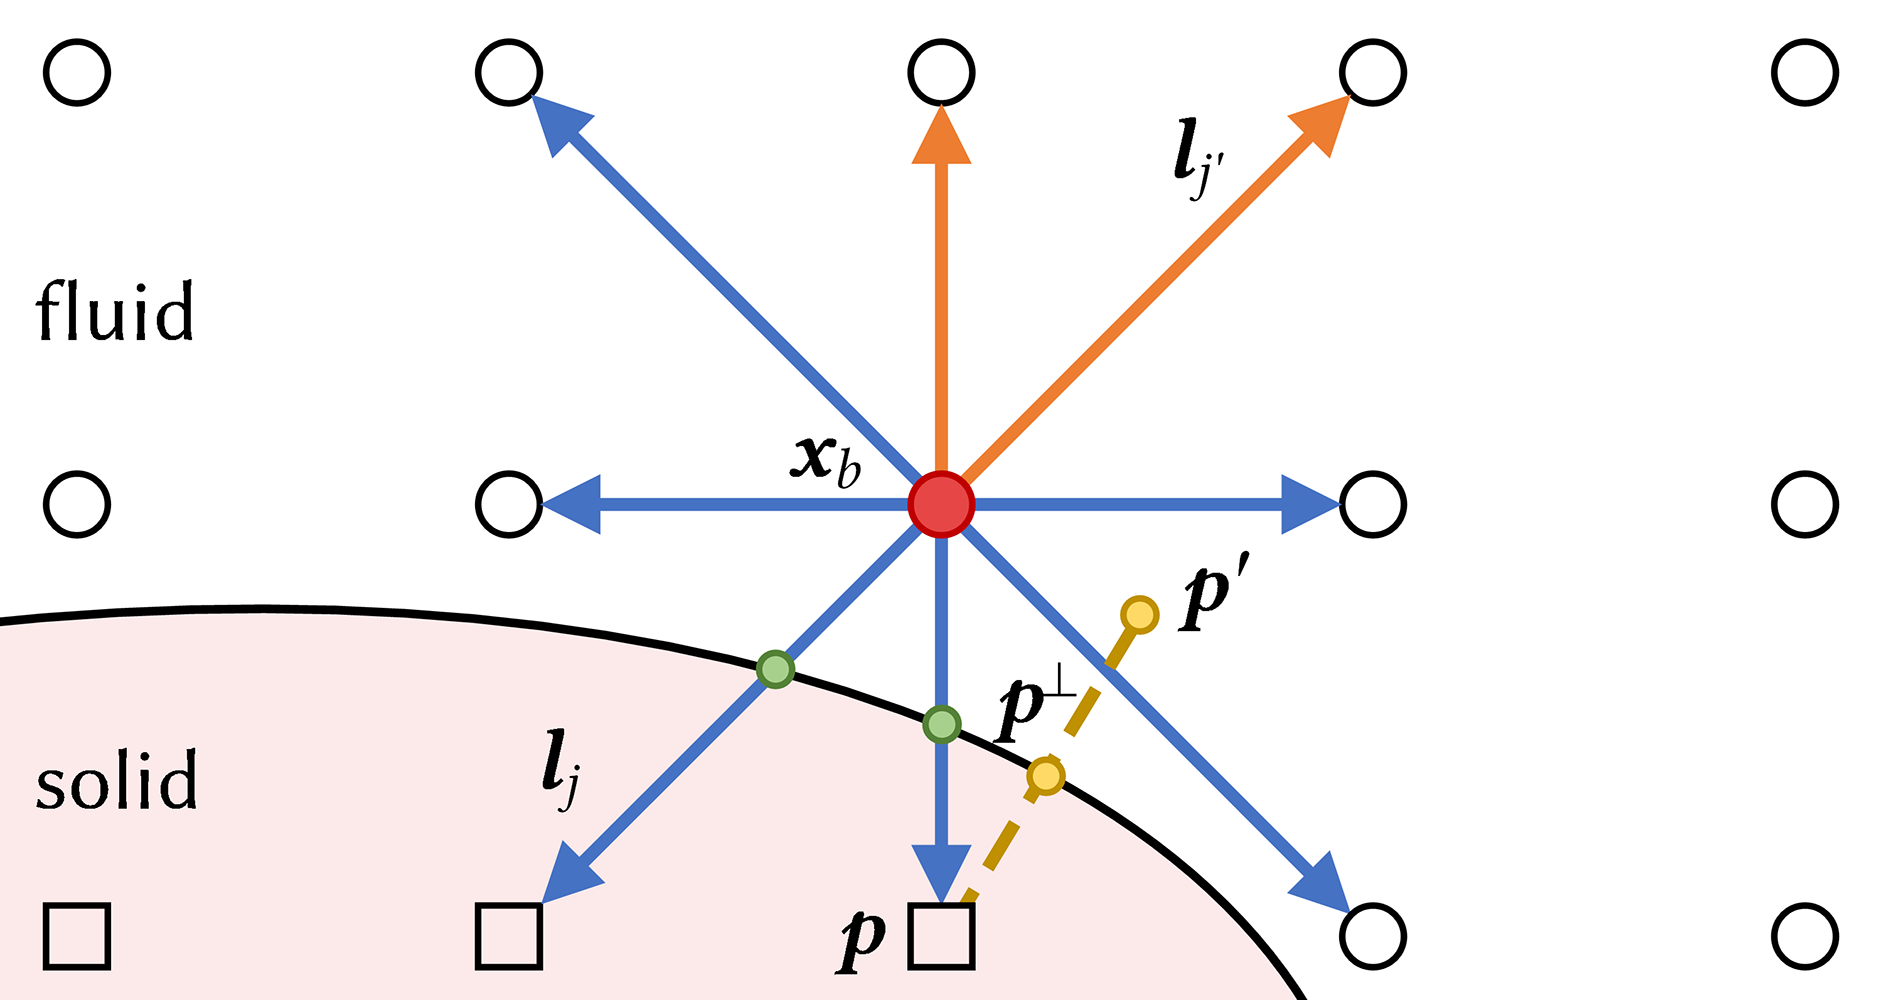
\includegraphics[width=0.68\columnwidth]{figures/bounce_back_scheme.png}
    \bicaption[固体边界的简单反弹方法与锐利界面浸入边界法]{固体边界的简单反弹方法与锐利界面浸入边界法。在迁移过程中,固体边界附近的流体格点$\bm{x}_b$ (图中标为红色圆圈) 的一部分分布函数$f_{j'}$ (图中标为橘色箭头) 是未知的,因为格点$\bm{x}_b-\bm{l}_{j'}$在固体内部 (图中标为方框),从而需要使用线段$\bm{x}_b$至$\bm{x}_b-\bm{l}_{j'}$与边界的交点 (图中标为绿色圆圈) 的速度$\bm{u}_s$来实现简单反弹边界处理,或$\bm{p}^\perp$与$\bm{p}'$点来实现锐利界面浸入边界处理。}{Simple bounce-back scheme and sharp-interface immersed boundary near fluid-solid boundary. During streaming, some of the distribution functions $f_{j'}$ (corresponding to the orange links) at the fluid node $\bm{x}_b$ (red circle) near a solid boundary are unknown, since the node at $\bm{x}_b-\bm{l}_{j'}$ is located inside the solid region (shown as boxes), requiring a bounce-back scheme using the velocity $\bm{u}_s$ of the boundary velocity at the intersection point (green circles) between the line segment from $\bm{x}_b$ to $\bm{x}_b-\bm{l}_{j'}$ and the solid boundary, or sharp-interface immersed boundary using $\bm{p}^\perp$ and $\bm{p}'$.}
    \label{img:bounce_back_scheme}
\end{figure}

\subsection{插值反弹边界}
简单反弹边界的一个问题是只有边界在速度方向中点时,边界处理的精度才可达到二阶。边界处于其他位置时,边界处理的精度只有一阶。
针对这一问题,插值反弹边界被提出~\citep{Bouzidi-2001},通过考虑边界到格点的距离,进行分布函数的插值:
\begin{equation}\label{eq:ibb_2001}
    f_i(\mathbf{x}_B, t+1) = 
    \begin{cases}
        2 q f^{*}_{\bar{\imath}}(\mathbf{x}_B, t)+(1-2 q) f^{*}_{\bar{\imath}}(\mathbf{x}_{F}, t), & q < 0.5, \\
        \frac{1}{2 q} f^{*}_{\bar{\imath}}(\mathbf{x}_B, t)+\frac{2 q-1}{2 q} f^{*}_i(\mathbf{x}_B, t), & q \geq 0.5,
    \end{cases}
\end{equation}
其中$q=\|\mathbf{x}_B - \mathbf{x}_W\|/\|\bm{c}_i\|$是边界点到边界的归一化距离,这里我们只考虑了静态边界的情况,在动态边界中可以如公式~\ref{eq:bounce-back} 中一样添加动量项。

在引入基于距离的插值后,反弹边界可以达到二阶精度,但是依然有一些问题。首先是公式~\ref{eq:ibb_2001} 引入了邻居点参与计算,对于GPU实现会降低数据访问效率。其次,当处理复杂外形的几何时,格点可能处于两个边界之间,导致找不到邻居点从而无法完成边界处理。最后,如第~\ref{sec:1_related_works_LBM} 节所介绍的,IBB在~\citet{Bouzidi-2001} 提出这一方法后逐渐发展成为了一类方法,之后的工作提出了诸多不同的构造形式,甚至参数化的构造。这些不同的构造的性能与精度均有所区别。关于这一部分我们将在第~\ref{chap:sig23} 章中继续讨论。

\subsection{浸入边界法}
浸入边界法 (Immersed Boundary Method,IBM) 是一个在LBM被经常采用的边界处理方法,其一般通过施加惩罚力实现边界条件~\citep{patel2018diffuse,mittal-2008,Li-2020}。在浸入边界法的诸多变种中,扩散边界浸没边界法 (Diffuse-Interface Immersed Boundary Method, DI-IBM) 与锐利界面浸入边界法 (Sharp-Interface Immersed Boundary Method, SI-IBM)~\citep{mittal-2008} 是最为广泛应用的。我们首先讨论扩散边界浸没边界法。

基于IBM的边界条件均使用预测-修正的思路,即首先忽视固体作用进行流体仿真,之后使用惩罚力对不满足固体边界条件的流体进行修正。在DI-IBM中,惩罚力施加在边界上,所以首先需要对固体表面进行均匀采样。然后对每一个采样点$\mathbf{x}_s$,通过插值得到该点的流体动量$\mathbf{m}_f$。这是通过基于核函数插值实现:
\begin{align}
    \begin{split} 
\boldsymbol{m}_{f}\left(\boldsymbol{x}_{s}\right) & =\int \boldsymbol{m}_{f}(\boldsymbol{x}) \, \delta(\boldsymbol{x}-\boldsymbol{x}_{s}) d \boldsymbol{x} \\
& \approx \sum_{\boldsymbol{x}_{f} \in \mathcal{D}_{s}} \boldsymbol{m}_{f}(\boldsymbol{x}_{f}) \, \bar{\delta}(\boldsymbol{x}_{f}-\boldsymbol{x}_{s}) \Delta v ,
    \end{split}
\end{align}
其中$\mathcal{D}_{s}$是$\boldsymbol{x}_{s}$周围格点的集合,$\boldsymbol{m}_{f}(\boldsymbol{x}_{f})=\rho(\boldsymbol{x}_{f})\boldsymbol{u}(\boldsymbol{x}_{f})$是格点$\boldsymbol{x}_{f}$的动量,$\Delta v=\Delta x^3$,$\Delta x$是网格大小。$\bar{\delta}\left(x_{f}-x_{s}\right)$是狄拉克 (Dirac) $\delta$ 函数的平滑近似,可被视为插值的核函数。这里我们得到的流体表面的动量$\boldsymbol{m}_{f}\left(\boldsymbol{x}_{s}\right)$并不能满足固体边界条件,所以我们要在该点施加一个惩罚力进行修正:
\begin{equation}
    \boldsymbol{F}_{f \rightarrow s}\left(\boldsymbol{x}_{s}\right)=\left(\boldsymbol{m}_{f}(\boldsymbol{x}_{s})-\rho \boldsymbol{v}_{s}(\boldsymbol{x}_{s})\right) / \Delta t ,
\end{equation}
其中$\boldsymbol{v}_{s}\left(\boldsymbol{x}_{s}\right)$是$\boldsymbol{x}_{s}$点的固体速度。而因为力最终要施加到流体格点上,我们需要把$\boldsymbol{F}_{f \rightarrow s}\left(\boldsymbol{x}_{s}\right)$扩散到周边的流体格点上,每个格点$\boldsymbol{x}_{f}$上面的力是
\begin{align}
    \begin{split}
\boldsymbol{F}_{s \rightarrow f}\left(\boldsymbol{x}_{f}\right) & =-\int \boldsymbol{F}_{f \rightarrow s}(\boldsymbol{x}) \, \delta(\boldsymbol{x}-\boldsymbol{x}_{f}) d \boldsymbol{x} \\
& =-\sum_{\boldsymbol{x}_{s} \in \mathcal{D}_{f}} \boldsymbol{F}_{f \rightarrow s}(\boldsymbol{x}_{s}) \, \bar{\delta}(\boldsymbol{x}_{s}-\boldsymbol{x}_{f}) \Delta v ,
    \end{split}
\end{align}
其中$\mathcal{D}_{f}$是格点$\boldsymbol{x}_{f}$周边的采样点集合。

\begin{figure}[!tb]
    \centering
      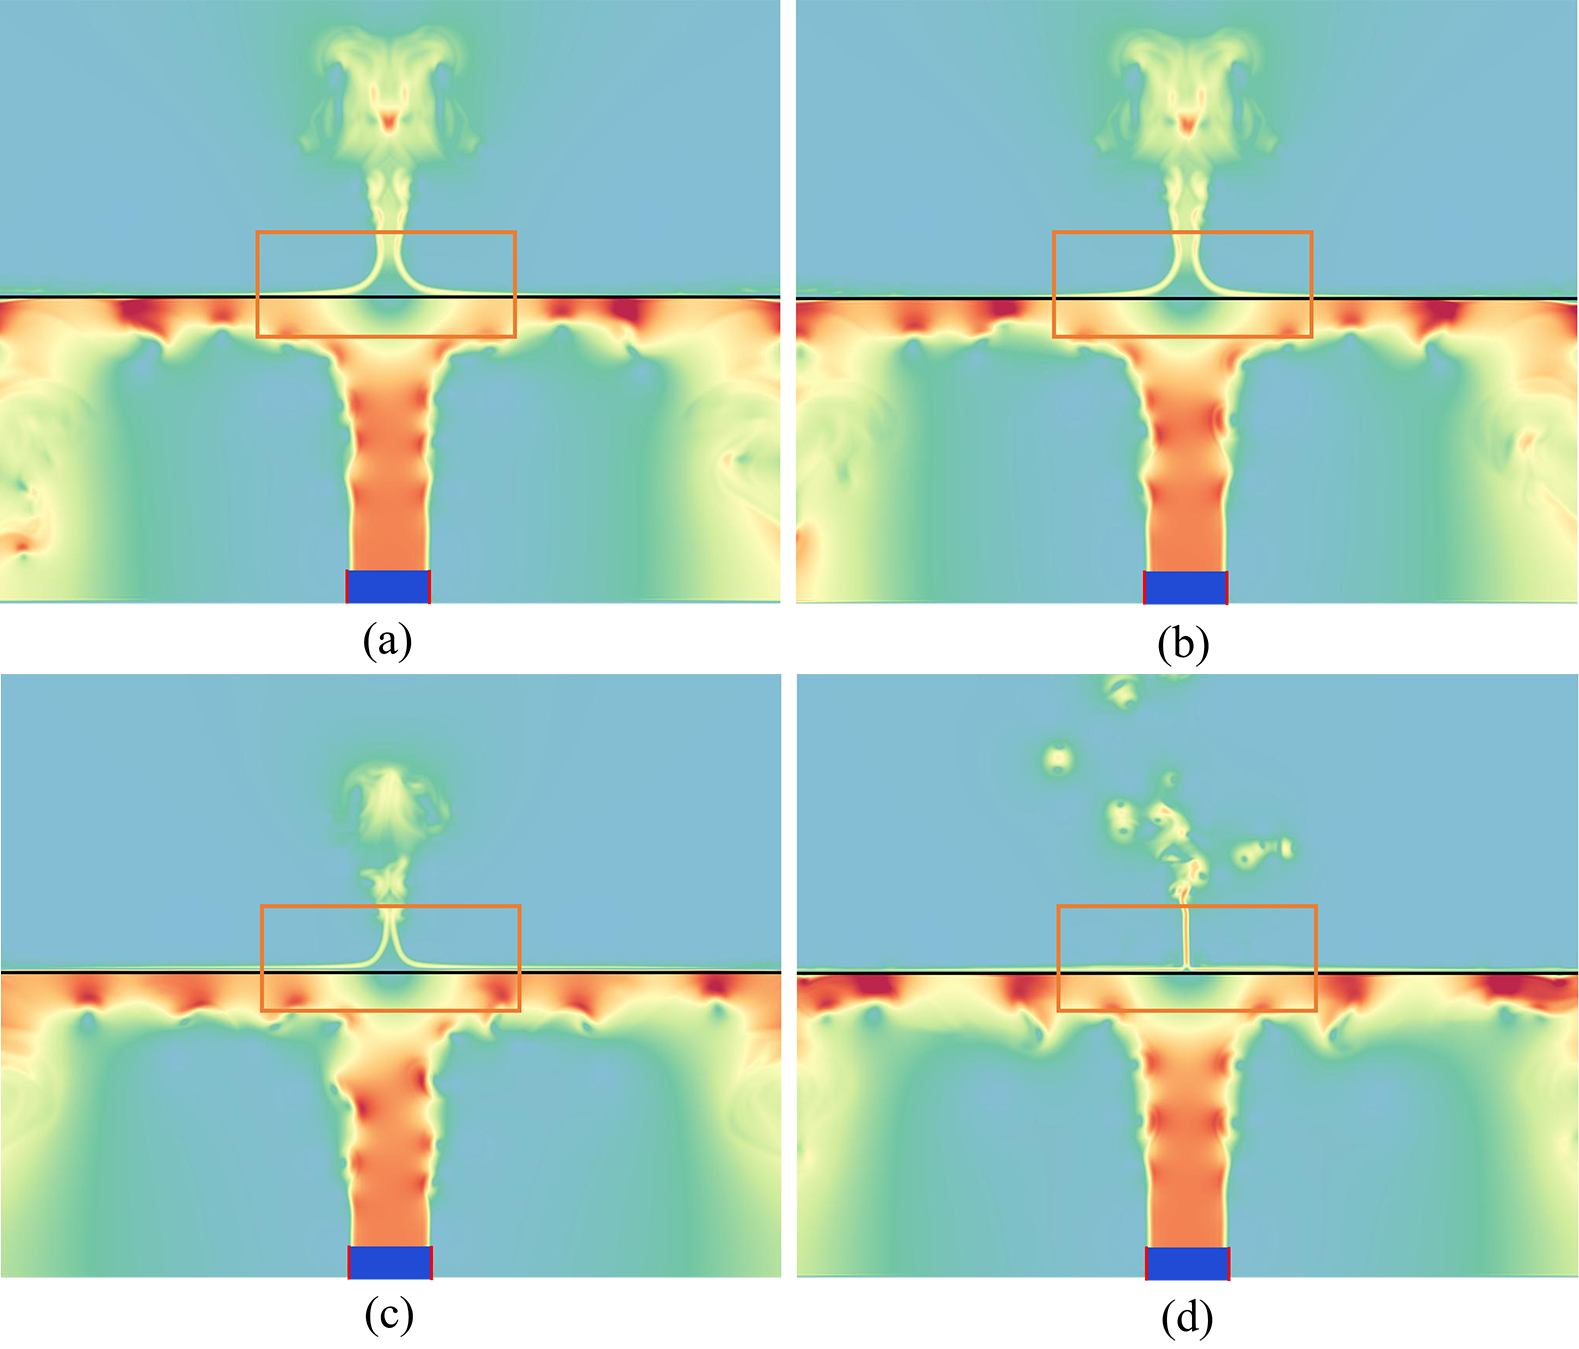
\includegraphics[width=0.8\columnwidth]{figures/leakage.png}
    \bicaption[浸入边界法的流体泄露问题]{浸入边界法的流体泄露问题。我们用一个薄板将二维的流体域分为两半,并在域的下方放置一个喷射流入口,这个喷射流在使用IBM作为边界条件仿真时会错误地流入域的上方 (见橘色方框)。其中,(a) 使用扩散边界浸没边界法~\citep{patel2018diffuse},
    (b) 使用迭代扩散边界浸没边界法~\citep{zhang2016accuracy},
    (c) 使用锐利界面浸入边界法~\citep{seo-2011sharp},
    (d) 使用基于分布函数修正的浸入边界法~\citep{tao-2018}。}{Fluid leakage caused by immersed boundary method. If a thin shell separates a 2D domain into two chambers, a jet in the lower chamber is erroneously leaking into the upper chamber (see the boxed regions) for
		(a) the diffuse-interface immersed boundary method~\citep{patel2018diffuse} ,
		(b) the iterative diffuse-interface immersed boundary method~\citep{zhang2016accuracy},
		(c) the sharp-interface immersed boundary method~\citep{seo-2011sharp}, and
		(d) the distribution function correction-based immersed boundary method~\citep{tao-2018}.}
    \label{img:leakage}
\end{figure}

而锐利界面浸入边界法在构造惩罚力的方法上有所不同,该方法的图示可见图~\ref{img:bounce_back_scheme}。
对于边界点,SI-IBM首先重建相邻固体点的分布函数 (在图~\ref{img:bounce_back_scheme} 中标为方框)。之后将该格点投影到固体边界上 (在图~\ref{img:bounce_back_scheme} 中标为$\bm{p}^\perp$),然后沿着法向$\bm{p}^\perp\!-\!\bm{p}$方向求得一个镜像点$\bm{p}'$。$\bm{p}'$的宏观速度可在固体边界的一侧通过周围点插值得到。因为固体点的速度$\bm{u}_b(\bm{p}^\perp)$是已知的,我们可以容易地计算出$\bm{p}$点的速度$\bm{u}^*(\bm{p}) = 2\bm{u}_b(\bm{p}^\perp) - \bm{u}(\bm{p}')$。显然这个速度会与$\bm{p}$点现有的宏观速度$\bm{u}(\bm{p})$有一个速度差$\Delta\bm{u}(\bm{p}) = \bm{u}^*(\bm{p}) - \bm{u}(\bm{p})$。这个速度差可以构成一个惩罚力$\bm{F}(\bm{p}) = \rho\Delta\bm{u}(\bm{p})$来修正$\bm{p}$点的流体速度。SI-IBM的一个优势是通过插值,固体边界的大速度梯度会被压制,从而提升稳定性。

虽然IBM的浸没特性使其可以较为容易地实现双向流固耦合,但是IBM并不适合用来处理亚网格尺度的物体的边界,原因是IBM中速度的传播经常会跨过薄物体,造成流体泄露,一个具体的例子可见图~\ref{img:leakage}。

\section{总结与讨论}
在本章中,我们主要介绍了LBM的理论背景,与碰撞模型和边界处理部分的具体实现形式。

对于边界处理部分,我们在第~\ref{sec:boundary_treatment} 节介绍了多个边界处理形式与存在的问题。我们认为目前的流体仿真主要面向两种不同的需求,一类是更注重在复杂场景下高效求解,而不是物理精度,如制作视觉动画;而另一类是更注重求解的精度,可以允许更长的求解时间,如工程应用。在前一类需求中,实现难度更低、前处理需求简单的简单反弹边界与浸入边界法更为适用,不过它们有很强的局限性,即难以在湍流中处理复杂几何,如亚网格物体。而对后一类需求,插值反弹边界作为目前最精准的边界处理,依旧难以在超高雷诺数下实现湍流边界层的准确仿真。
我们在第~\ref{chap:siga21} 章中提出可处理复杂几何的混合边界处理方法,并在第~\ref{chap:sig23} 章中提出新的插值反弹边界形式,以解决上述两类需求所面临的问题。

对于碰撞部分,我们在第~\ref{sec:bg_collision} 节讨论了精度与高阶松弛系数之间的关系与高阶松弛系数的一些优化方法。总的来看,累积量碰撞模型的理论误差与数值表现相比其它模型都更有优势。但是我们注意到,目前累积量模型的高阶松弛系数只在3阶上有优化的形式。我们认为在更高阶的累积量上优化松弛系数可以进一步提升方法的精度与稳定性。第~\ref{chap:sig23} 章中,我们基于熵优化的想法,介绍并讨论了如何完成这一过程。

此外,为了精准地计算物理量,还需要很多方法上的整体考量。如使用流体仿真对汽车进行数值风洞实验,汽车被放置在地面上时会与地面产生一个非常狭窄的空间。这个空间中的流体动态对最终的物理量有着很大的影响。同时,考虑到有限的计算资源,如何高效构建多分辨率计算网格也是十分重要的问题。这些在利用LBM进行工程应用计算时需要解决的问题,在目前的文献资料中鲜有讨论。这些内容我们也在第~\ref{chap:sig23} 章中进行讨论。